\chapter{Contextualización}

\section{Análisis del problema}

    \subsection*{Definición y características clínicas del queratocono}

        El queratocono es una enfermedad ocular en la que la córnea (la parte transparente y curva en la superficie del ojo) se debilita y adelgaza progresivamente, deformándose hasta tomar una forma cónica en lugar de su curvatura normal (Figura~\ref{fig:comparacion_corneas}). Esto altera la manera en que la luz ingresa al ojo, generando visión borrosa y distorsionada que empeora con el tiempo si no se detecta en etapas iniciales \cite{queratocono}.

        \vspace{-0.5 cm}
        \begin{figure}[H] \centering
            \begin{subfigure}[b]{0.45\textwidth} \centering
                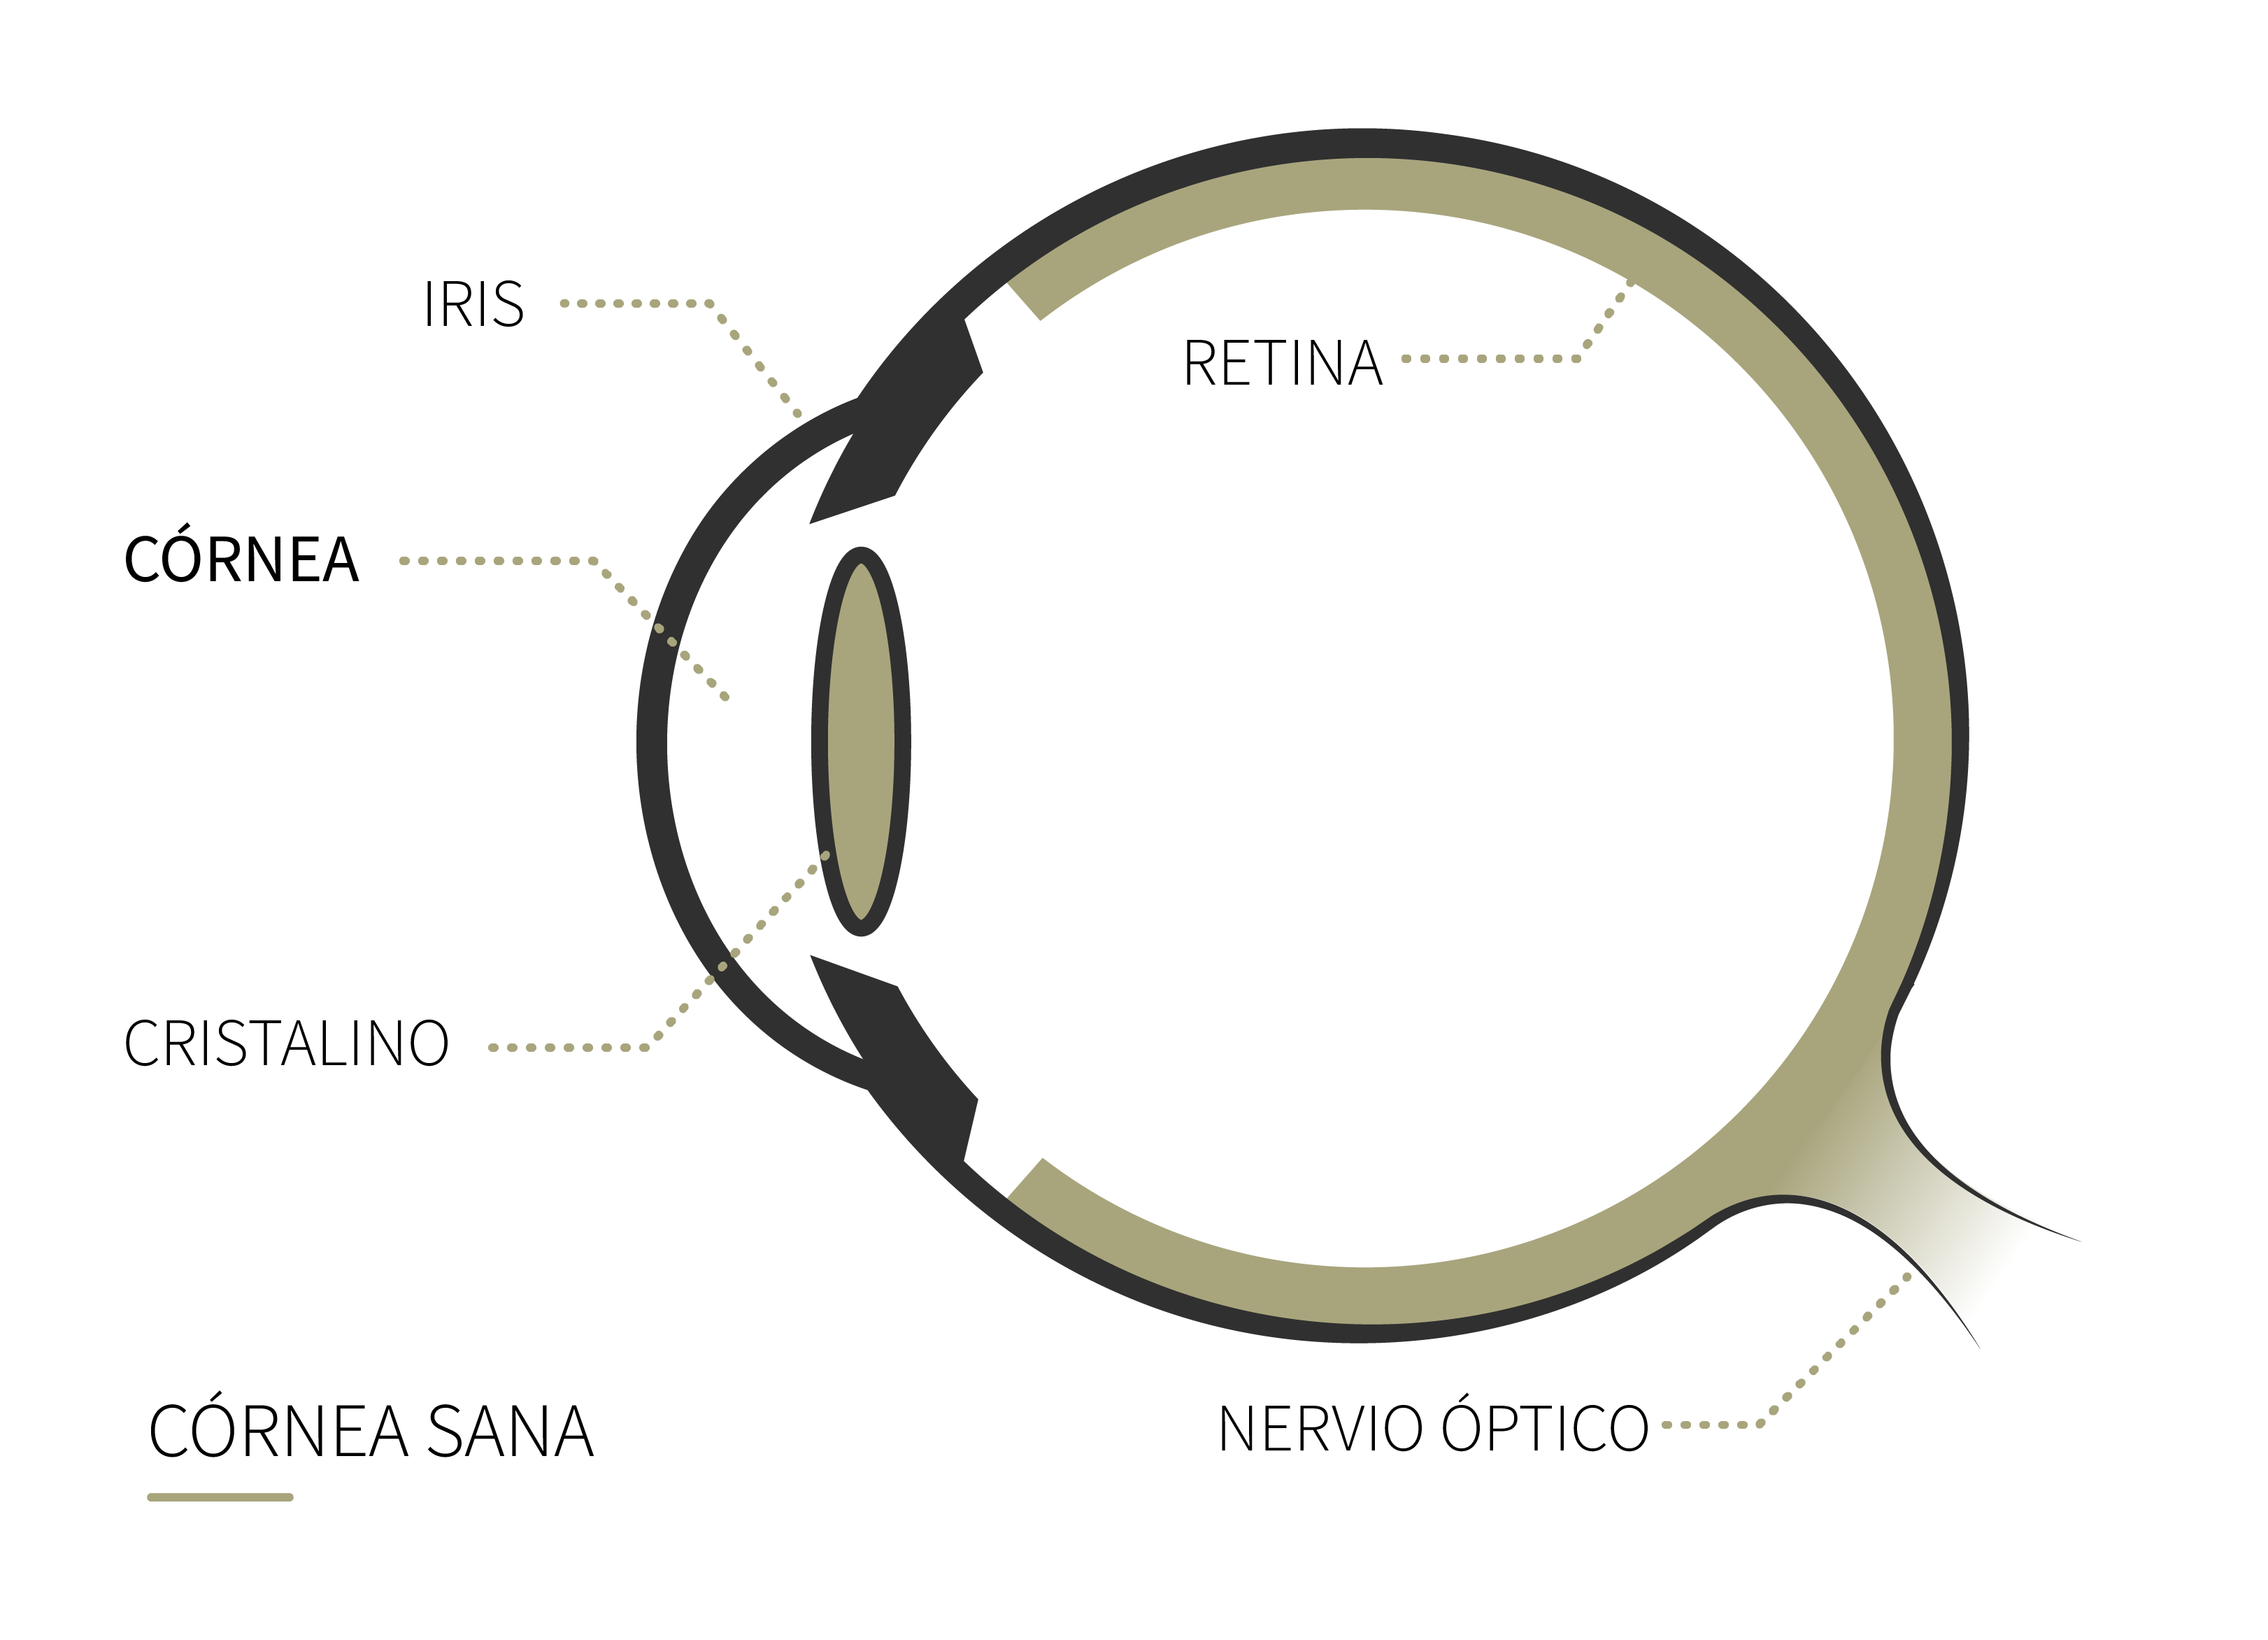
\includegraphics[width=\textwidth]{img/queratocono_deformacion_a.png} 
                \caption{Córnea sana}
                \label{fig:cornea_a}
            \end{subfigure}
            \hspace{-1 cm}
            \begin{subfigure}[b]{0.45\textwidth} \centering
                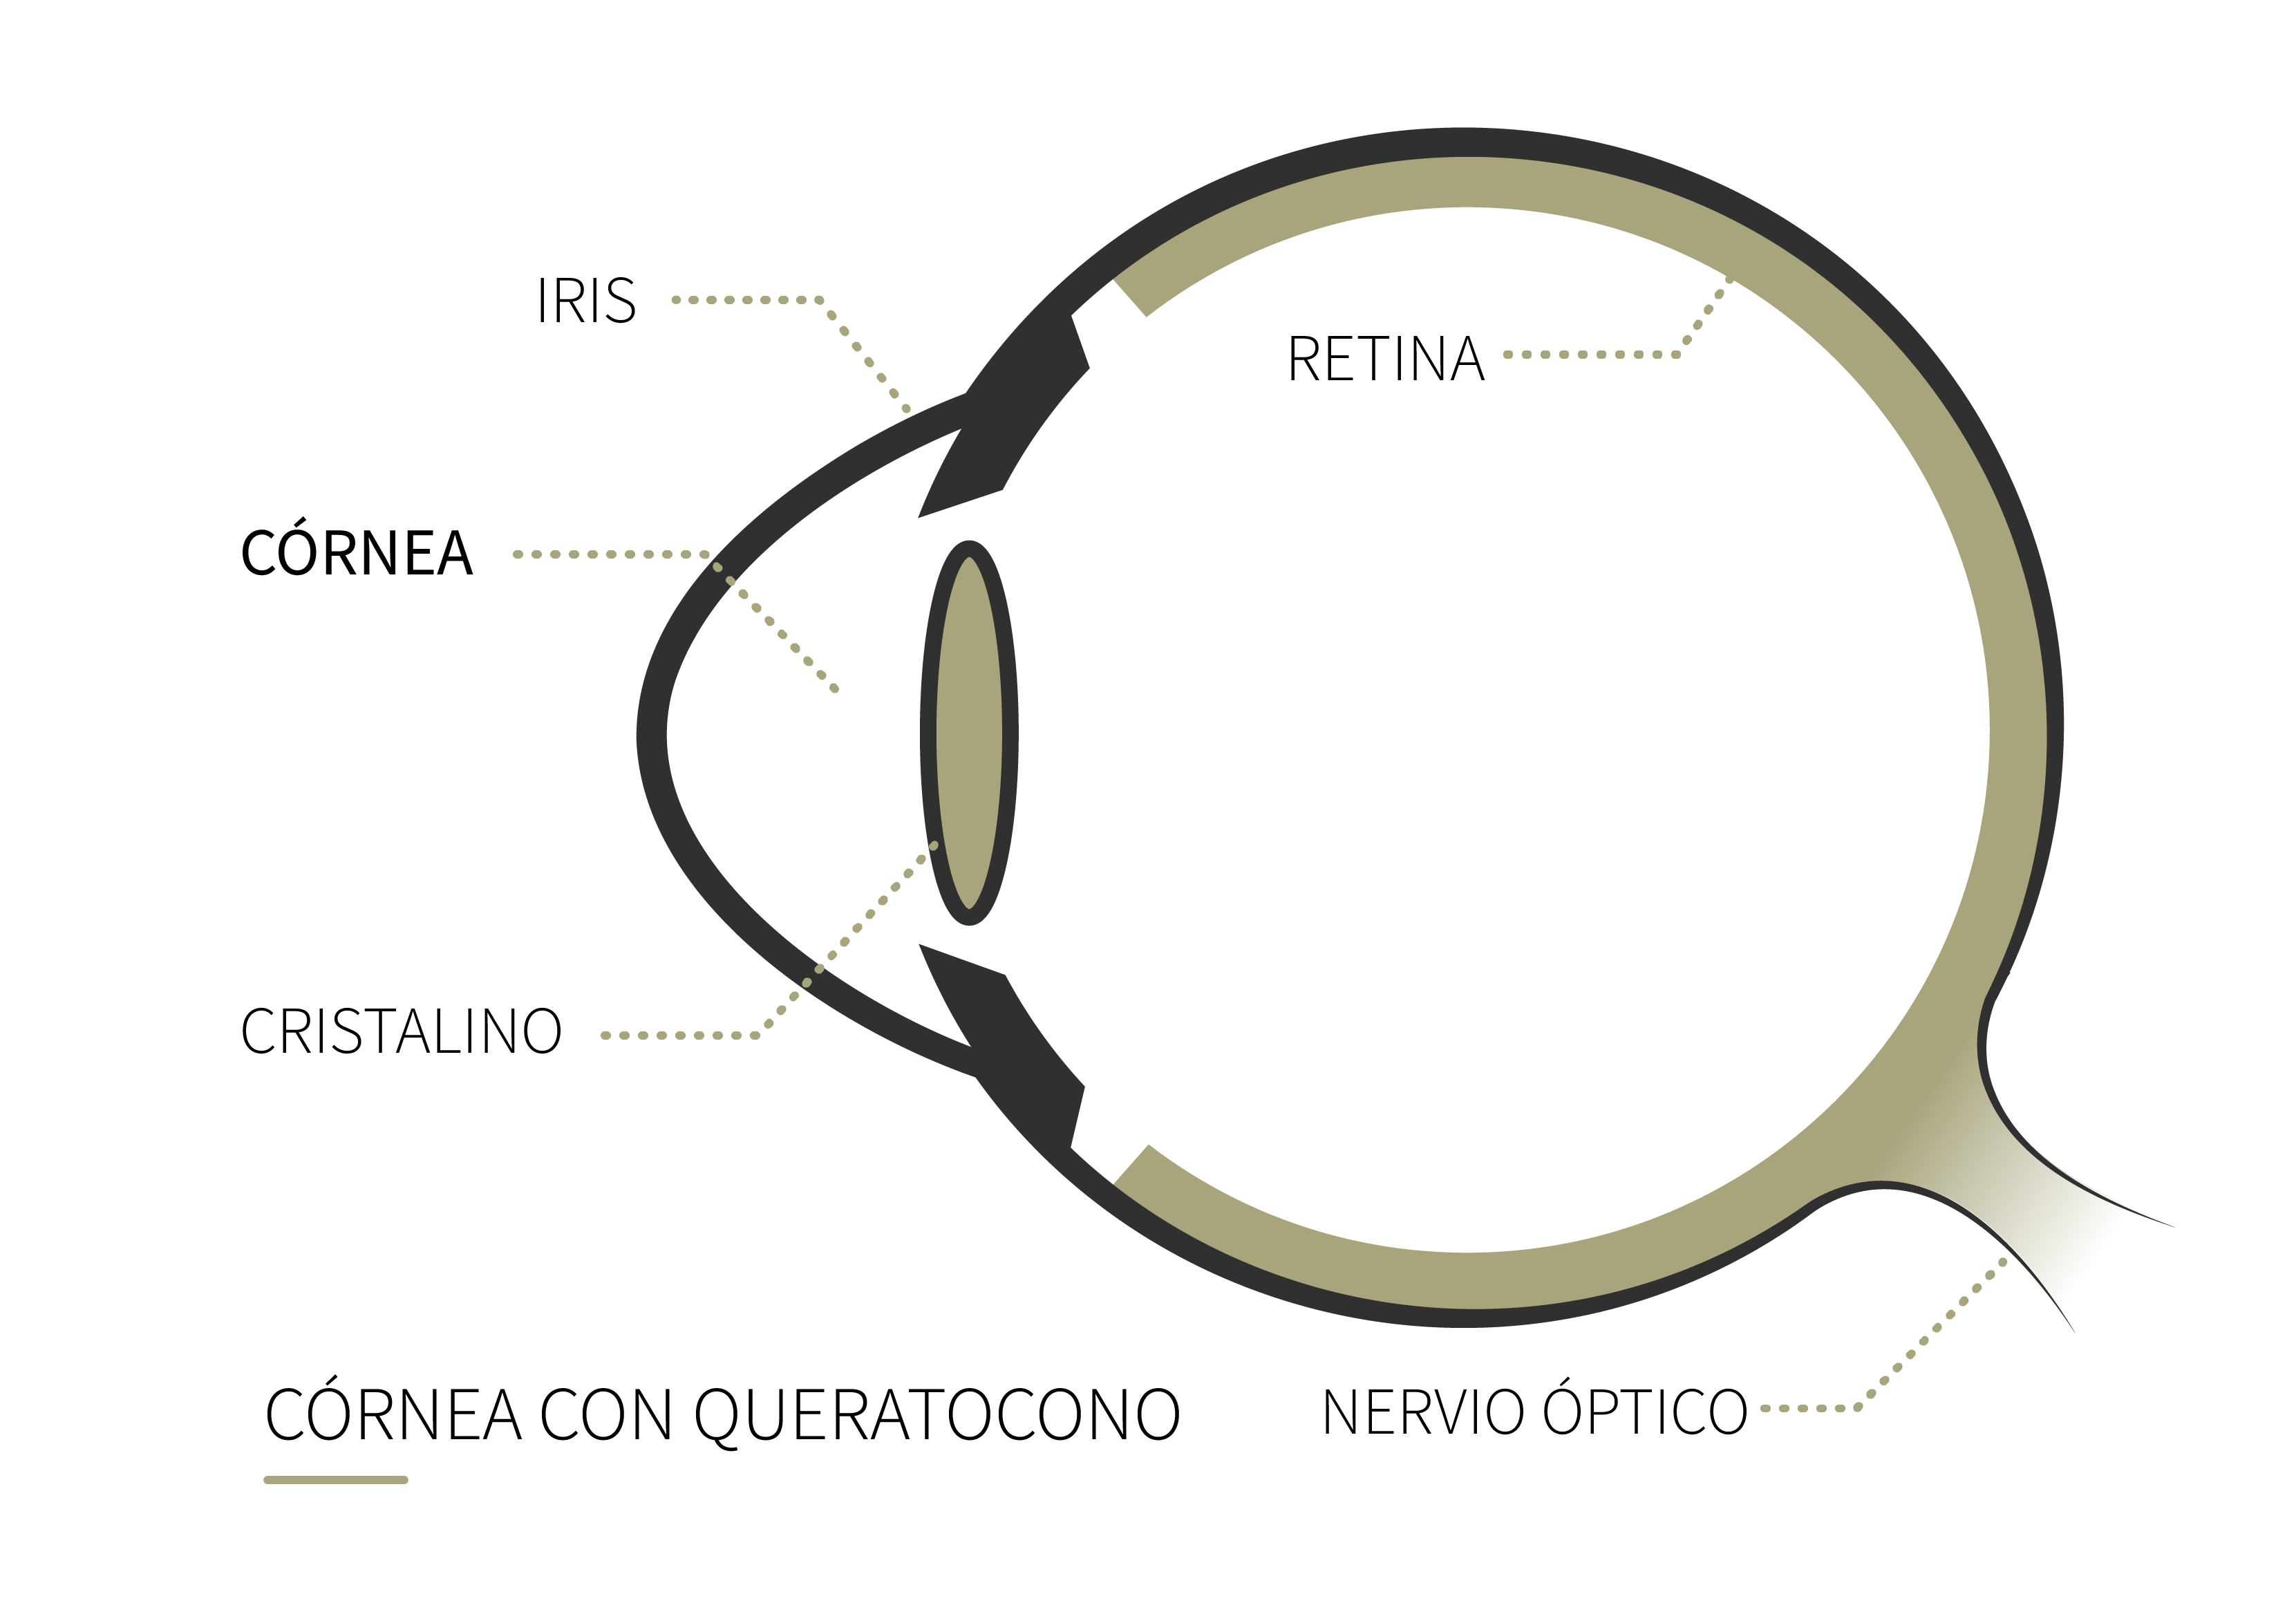
\includegraphics[width=\textwidth]{img/queratocono_deformacion_b.png}
                \caption{Córnea con queratocono}
                \label{fig:cornea_b}
            \end{subfigure}
            \caption{Comparación anatómica entre córnea sana y córnea con queratocono.}
            \label{fig:comparacion_corneas}
        \end{figure}

    \par\vspace{-0.5 cm}
    \subsection*{El desafío del diagnóstico temprano}
    
        El queratocono presenta la dificultad de que sus manifestaciones iniciales son sutiles y pueden confundirse con miopía o astigmatismo común. Esta interpretación está condicionada por la experiencia del profesional, lo que aumenta la probabilidad de errores, especialmente en etapas subclínicas donde la patología se manifiesta de forma discreta y no resulta evidente en una revisión superficial del estudio.
    
        Esta situación se ve agravada por la rápida aparición y avance de la enfermedad en edades tempranas de los pacientes, lo que representa un punto crítico en cuanto al tiempo de diagnóstico y tratamiento. La demora en la detección puede derivar en una progresión irreversible del daño corneal, llegando en estadios medios y avanzados a necesitar intervención quirúrgica para no perder la visión \cite{deteccion_temprana}.
        
        La interpretación visual de mapas topográficos y tomográficos puede derivar en diagnósticos confusos o tardíos, particularmente en manos de médicos con menos experiencia, lo que fundamenta la necesidad de generar herramientas de asistencia al diagnóstico basadas en Inteligencia Artificial (IA) para estandarizar los criterios de evaluación y reducir la variabilidad inherente al proceso \cite{queratocono_ia}.

    \subsection*{Indicadores cuantitativos}

        Se estima que afecta a más de 23,7 millones de personas a nivel mundial, con una prevalencia global de 289 casos por cada 100.000 habitantes~\cite{prevalencia_kc}. A pesar de los avances en imagenología corneal, la detección de estadios subclínicos es un desafío dado que los sistemas de IA alcanzan una sensibilidad del 90\,\% en estos casos, frente al 98,6\,\% en casos ya manifiestos, es decir que uno de cada diez ojos con queratocono subclínico pasa desapercibido, contra menos de dos de cada cien con deformación más avanzada~\cite{sensibilidad_ia_subclinica}.
        
        Esta dificultad se traduce en demoras diagnósticas de hasta 2,9 años entre la primera consulta optométrica y la derivación oftalmológica~\cite{demora_diagnostica}, retraso que resulta crítico considerando que hasta el 88\,\% de los casos de ectasia corneal postquirúrgica\footnote{Adelgazamiento y encorvamiento progresivo de la córnea posterior a una cirugía refractiva, cuando el tejido remanente pierde la resistencia necesaria para sostener la presión intraocular. Puede llegar a requerir un trasplante.} se atribuyen a ojos queratocónicos que no fueron detectados a tiempo~\cite{falsos_negativos_ectasia}.

    \subsection*{Impacto local}
    
        En la provincia de Misiones, se ha reportado un aumento de casos de queratocono en la ciudad de Oberá~\cite{misiones}. El problema real es que la infraestructura diagnóstica se concentra en Posadas y Alem donde, para un paciente de zonas remotas de la provincia, una consulta podría ser su única oportunidad de detección dados los costos de traslado, lo que evidencia la relevancia regional de la problemática. 
        
        Un soporte a la decisión clínica actuaría como una herramienta de ayuda para referenciar los criterios de evaluación, pudiendo reducir el riesgo de errores diagnósticos y permitiendo intervenciones oportunas para preservar la visión de los pacientes.
        
    \subsection*{Riesgos de implementación y barreras normativas}
    
        Al tratarse de una aplicación en el ámbito de la salud, la implementación de este sistema conlleva riesgos críticos que deben ser tenidos en cuenta. La integración de modelos de IA exige una rigurosa validación externa o local. Este proceso es fundamental para contrastar el rendimiento del algoritmo con la realidad clínica diaria. Esto permite evaluar y documentar de manera rigurosa la fiabilidad y eficacia del sistema bajo las condiciones y recursos de nuestra región.
    
        Por otro lado, la Disposición N.º 9688/2019 de la Administración Nacional de Medicamentos, Alimentos y Tecnología Médica (ANMAT) establece en su artículo 26 que todo \textit{software} que se encuadre en la definición de producto médico debe inscribirse en el Registro de Productores y Productos de Tecnología Médica~\cite{dispo_9688}, requisito que alcanza directamente a este sistema. La inscripción no certifica por sí sola que el producto sea seguro, sino que exige presentar los ensayos que respaldan el informe de Requisitos Esenciales de Seguridad y Eficacia, con una profundidad que depende de la clase de riesgo asignada según la Disposición ANMAT N.º 2318/2002~\cite{dispo_2318}.
        
        La responsabilidad legal de los datos locales recae en los oftalmólogos consultados, en su labor de anonimizar los estudios provistos. Por otro lado, los datos presentes en los \textit{datasets} internacionales~\cite{kaggle,zenodo,insight} ya vienen anonimizados previamente para su uso, garantizando la transparencia y validación clínica según la Ley N.º 25.326 de Protección de los Datos Personales, sancionada en el año 2000~\cite{ley_25326}.

\phantomsection
\par\vspace{-0.2 cm}
\section{Antecedentes}

    \par\vspace{-0.25 cm}
    \subsection*{Redes neuronales recurrentes (RNN)}

        Un antecedente fundamental es el modelo de aprendizaje profundo multimodal presentado por Shafi Balal en el congreso ESCRS 2025, abordando la problemática de que los médicos no pueden predecir con certeza qué pacientes progresan hacia estadios graves y cuáles son estables, saturando los servicios con seguimientos frecuentes. Su sistema utiliza redes neuronales recurrentes para analizar datos de solo dos visitas, logrando clasificar a los pacientes en grupos de bajo o alto riesgo de progresión a dos años~\cite{shafi_balal}.

        Este trabajo demuestra que es posible construir modelos predictivos con una cantidad reducida de información clínica y que es viable estratificar el riesgo de progresión. Sin embargo, requiere datos de más de una visita por paciente, información con la que no cuentan los conjuntos de datos disponibles para este proyecto. Por ello, la estratificación del riesgo de progresión se plantea como una línea de trabajo futuro (ver sección Alcance y limitaciones).

    \par\vspace{-0.1 cm}
    \subsection*{Redes neuronales convolucionales (CNN)}
    
        Por otro lado, el desarrollo del algoritmo KeratoDetect se enfoca en la dificultad de detectar el queratocono en etapas subclínicas. Este algoritmo demostró que los modelos basados en redes neuronales convolucionales pueden identificar patrones patológicos que el ojo humano podría omitir, procesando imágenes corneales para una clasificación binaria con alta precisión~\cite{kerato_detect}.

        Este antecedente se centra exclusivamente en el análisis de imágenes, sin incorporar datos clínicos del paciente ni integrarse a un sistema para oftalmólogos. Aun así, respalda el objetivo central del trabajo, la detección, y justifica la utilización de redes CNN para definir la arquitectura de procesamiento.

    \par\vspace{-0.1 cm}
    \subsection*{Herramientas médicas e investigación}
    
        En el ámbito local, no existen competidores directos con un software como producto médico específico para queratocono en Argentina. El referente más cercano es Entelai~\cite{entelai}, una \textit{startup} líder en el país en la aplicación de IA para el análisis de imágenes médicas, cuyo modelo de validación asistida permite a los médicos procesar informes con rapidez. A nivel internacional, proyectos como KERAFound y el sistema multi-agente AEYE~\cite{aeye} están evolucionando desde la investigación académica hacia las herramientas comerciales de aplicación.
    
        Mediante estos antecedentes se demuestra que es posible predecir la enfermedad y estratificar su riesgo basándose en imágenes topográficas y datos clínicos relevantes. Además, la industria está interesada en la adopción de aplicaciones médicas para el apoyo en el flujo de trabajo e investigar estas herramientas.

    \subsection*{\textit{Vision Transformers}}

        En paralelo al uso de arquitecturas convolucionales, distintos trabajos recientes han incorporado \textit{Vision Transformers} (ViT) para el análisis de queratocono, superando las limitaciones de las CNN en la captura de dependencias espaciales de largo alcance dentro de la imagen corneal. 

        Abdelmotaal et al. presentaron un modelo híbrido Transformer-CNN para la detección automática de queratocono a partir de videos de deformación corneal dinámica basados en Scheimpflug~\cite{abdelmotaal_vit}, mientras que otro trabajo propuso la fusión de múltiples modelos preentrenados junto con una arquitectura transformer para la clasificación de imágenes corneales~\cite{vit_fusion_kcn}. Asimismo, se desarrolló un modelo transformer multi-fuente que integra topografía, aberrometría y datos tabulares para predecir la progresión de la enfermedad~\cite{vit_multisource}. 
        
        Estos antecedentes evidencian una tendencia hacia arquitecturas más complejas que las CNN tradicionales. Sin embargo, dado el volumen de datos disponibles y las limitaciones de desarrollo del presente trabajo, la adopción de \textit{Vision Transformers} resulta como una alternativa a explorar pero no obligatoria, siendo una limitación del enfoque actual o una línea de trabajo futura.

    \subsection*{Modelos fundacionales}

        Otro antecedente relevante es RETFound, el primer modelo fundacional (\textit{foundation model}) en oftalmología, entrenado mediante aprendizaje autosupervisado (\textit{masked autoencoder}) sobre 1,6 millones de imágenes retinianas no etiquetadas, logrando superar a modelos preentrenados en ImageNet en tareas de diagnóstico y pronóstico con una cantidad reducida de datos etiquetados~\cite{retfound}. Esta línea de trabajo fue posteriormente extendida por el \textit{Global RETFound Consortium}, que propuso un modelo fundacional médico de alcance global~\cite{retfound_global}.
        
        Este tipo de modelos demuestra que es posible reducir significativamente la dependencia de grandes volúmenes de datos etiquetados mediante preentrenamiento a gran escala. Sin embargo, su implementación requiere capacidad de cómputo y acceso a \textit{datasets} masivos que exceden el alcance y las limitaciones de desarrollo del presente trabajo, por lo que su exploración se plantea como trabajo futuro.

    \subsection*{Comparativa de los antecedentes}

        Los antecedentes resuelven partes del problema de forma aislada: algunos analizan solo imágenes, otros se encuentran en fase de investigación y los productos comerciales no ofrecen un módulo específico para queratocono. Ninguno combina la detección a partir de imágenes y datos clínicos con la explicación visual de cada predicción, en una herramienta accesible pensada para el flujo de trabajo del oftalmólogo y el marco regulatorio local.

        \begingroup \setstretch{1.1}
        \begin{longtblr}[
            caption = Tabla comparativa de antecedentes y aporte diferencial de la propuesta,
            label = tabla_antecedentes_comparativa
            ]{
                colspec = {Q[c,m,2.75cm] X[l,m] X[l,m]},
                cells = {font=\small},
                row{1} = {bg=gray!15, font=\small\bfseries, halign=c},
                hlines, vlines,
                rowsep = 3pt, colsep = 5pt
            }
            
            Referencia & Aporte & Limitación \\
            
            Shafi Balal
            & Clasificación binaria del riesgo a dos años con solo dos visitas. Utiliza RNN.
            & No aborda detección temprana ni se integra a un sistema médico. \\
            
            KeratoDetect
            & Detección binaria subclínica para reducir la subjetividad. Utiliza CNN.  
            & Analiza solo imágenes y no se integra a un sistema médico. \\
            
            Entelai
            & Plataforma comercial líder en Argentina para la agilización de informes médicos. 
            & Solución general, no posee un módulo específico ni adaptado para queratocono. \\
            
            KERAFound / AEYE
            & Investigaciones académicas con transición a herramientas de diagnóstico. 
            & Diseñados para sistemas internacionales de alta gama, sin adecuación regulatoria. \\
            
            \textbf{Nuestro proyecto }
            & Detección temprana multimodal (imágenes y datos clínicos) con explicación visual, en una aplicación web accesible. Utiliza CNN.
            & Prototipo entrenado con un \textit{dataset} público. Requiere validación con muestras locales. \\
            
        \end{longtblr}
        \endgroup
        
\phantomsection
\par\vspace{-0.75 cm}
\section{Justificación}

    El proyecto se justifica por tres razones fundamentales que lo distinguen de las soluciones existentes y que responden a una necesidad concreta no resuelta en el mercado actual.

    En primer lugar, la accesibilidad, el sistema trabaja con los mapas corneales que exportan los equipos de topografía y tomografía ya instalados en los centros de salud, sin requerir \textit{hardware} de altísima gama, lo que facilita su adopción en la región, donde la infraestructura diagnóstica puede ser variada. El prototipo se desarrolla con mapas de equipos Orbscan, y su extensión a otros equipos disponibles localmente, como Pentacam y Sirius, se plantea como trabajo futuro.
    
    Seguidamente, la independencia y los costos, el proyecto propone un modelo de \textit{software} independiente, rompiendo con los ecosistemas cerrados y costosos de marcas como OCULUS\textsuperscript{\textregistered} o Topcon\textsuperscript{\textregistered}, cuyos sistemas de análisis dependen obligatoriamente de la adquisición de dispositivos propietarios, lo que genera una barrera de entrada para los que ya cuentan con equipos de otros fabricantes.
    
    Por último, la relevancia local, el proyecto aborda una problemática con evidencia clínica real en la región, con un aumento reportado de casos de queratocono en Oberá \cite{misiones}, lo que genera una necesidad concreta de herramientas diagnósticas asistidas por tecnología que no se encuentran disponibles en el mercado nacional.
    
    La solución técnica propuesta busca mitigar la subjetividad inherente a la interpretación de mapas corneales, reduciendo la dependencia de la experiencia del médico de turno y garantizando un diagnóstico más preciso y estandarizado independientemente de quién evalúe el estudio.
    
    Desde el punto de vista técnico, se trata de una adaptación innovadora de tecnologías conocidas, como redes neuronales convolucionales, algoritmos de explicabilidad y plataformas web modernas, a una necesidad clínica concreta no resuelta con los sistemas actuales.

    \subsection*{Impacto económico}

        Al no existir datos económicos sistematizados sobre el queratocono en Argentina, se plantea un análisis del costo de los estudios necesarios para la herramienta propuesta frente al de los tratamientos correspondientes a etapas avanzadas de la enfermedad. Para ello, tomamos en cuenta el nomenclador nacional de prácticas oftalmológicas de 2025~\cite{nomenclador_cao}, sin considerar descuentos como, por ejemplo, los de las obras sociales.
        
        Mientras que un estudio de topografía o tomografía corneal ronda los \$\,150.000, los procedimientos quirúrgicos representan un salto gigantesco en costo. El \textit{cross-linking} corneal y el implante de anillos intracorneales oscilan entre 3 y 3,3 millones de pesos por ojo, mientras que un trasplante de córnea puede superar los 10 millones de pesos por ojo considerando los costos de importación del tejido, cirugía y seguimiento postoperatorio. 
        
        Bajo este escenario, un sistema de detección temprana que evite o retrase la progresión hacia estas instancias quirúrgicas representaría un ahorro potencial considerable tanto para el paciente como para el sistema de salud, además de reducir la carga sobre los servicios de oftalmología especializada al filtrar los casos de bajo riesgo mediante una primera evaluación asistida.

\phantomsection
\par\vspace{-0.4 cm}
\section{Objetivos}

    \par\vspace{-0.15 cm}
    \subsection*{Objetivo general}
    
        Desarrollar un sistema de soporte a la decisión clínica, basado en algoritmos de inteligencia artificial sobre mapas corneales y datos clínicos, dirigido a los oftalmólogos para la detección temprana del queratocono y accesible mediante una aplicación web.

    \subsection*{Objetivos específicos}

        \begin{enumerate}[label=\textbf{\arabic*)},leftmargin=*]
            \item Analizar y preparar un conjunto de datos público y multimodal~\cite{zenodo}, que reúne mapas corneales y variables clínicas, caracterizando su composición y calidad antes del entrenamiento.

            \item Desarrollar y entrenar un modelo de aprendizaje profundo multimodal, basado en redes neuronales convolucionales, que combine los mapas corneales con las variables clínicas para identificar el queratocono, priorizando la reducción de falsos negativos.

            \item Integrar herramientas de inteligencia artificial explicable que proporcionen evidencia visual al oftalmólogo sobre las regiones corneales determinantes para cada predicción.

            \item Desarrollar una aplicación web que permita al oftalmólogo cargar los estudios del paciente, ejecutar el modelo y consultar un informe con el resultado y su explicación visual.
        \end{enumerate}

\phantomsection
\section{Alcance y limitaciones}

    Esta sección delimita qué demostrará el prototipo desarrollado en el marco del Proyecto Final Integrador (PFI) y qué aspectos quedan fuera de su alcance, de modo que los resultados que se presenten se correspondan con lo que el prototipo efectivamente puede comprobar.

    \subsection*{Alcance del prototipo}

        El prototipo funciona como una herramienta de apoyo: recibe la información de un estudio corneal, la procesa con un modelo de IA y devuelve un resultado que el oftalmólogo interpreta y valida. En concreto:

        \begin{itemize}[leftmargin=*]
            \item \textbf{Qué ingresa:} los cuatro mapas corneales de un ojo (axial, elevación anterior, elevación posterior y paquimetría), tal como los entrega un equipo Orbscan, junto con las variables clínicas del paciente: edad, sexo, astigmatismo, curvatura máxima de la córnea (K max), espesor corneal central y en su punto más delgado, y asfericidad anterior y posterior.

            \item \textbf{Qué procesa:} un modelo multimodal analiza las imágenes y los datos clínicos en conjunto y estima la probabilidad de que el ojo presente queratocono. A la vez, la técnica Grad-CAM marca sobre los mapas las regiones que más influyeron en esa estimación.

            \item \textbf{Qué entrega:} un informe con la clasificación del ojo (normal o con queratocono), el nivel de confianza del modelo y el mapa de calor que la justifica, consultable desde la aplicación web.
        \end{itemize}

        El entrenamiento y la evaluación se realizan con el \textit{dataset} público CornOrb~\cite{zenodo}, ya que las muestras locales se encuentran en proceso de solicitud a centros de salud de la región (ver capítulo Desarrollo). Si se obtienen durante el PFI, se incorporarán para una primera evaluación del modelo sobre datos regionales. El prototipo se considera terminado cuando el modelo esté entrenado y evaluado con ese conjunto de datos y la aplicación web permita ejecutarlo de punta a punta.

    \subsection*{Limitaciones}

        \begin{itemize}[leftmargin=*]
            \item \textbf{Disponibilidad limitada de grandes \textit{datasets}:} los conjuntos de datos públicos de queratocono son escasos y de tamaño moderado. CornOrb reúne 1.454 ojos de 744 pacientes, un volumen suficiente para entrenar y evaluar un prototipo, pero acotado frente al que requieren arquitecturas más complejas como los \textit{Vision Transformers} o los modelos fundacionales.

            \item \textbf{Falta de datos de carácter local:} las muestras de pacientes de Misiones se encuentran en proceso de solicitud y aún no se dispone de ellas. Hasta que se obtengan, el desempeño del prototipo solo podrá informarse sobre el conjunto de datos público. Aun si se incorporan durante el PFI, permitirán una evaluación preliminar sobre la población regional, pero no una validación clínica.

            \item \textbf{Validación en un único origen de datos:} todas las muestras de CornOrb provienen de un mismo tipo de equipo (Orbscan~3) y de centros de un mismo país. Para afirmar que el sistema funciona en la práctica clínica sería necesario validarlo en distintos centros de salud, con otros equipos y otros protocolos de adquisición.

            \item \textbf{Diferencias entre poblaciones y contextos clínicos:} los datos corresponden a pacientes de Argelia, por lo que las características de la población y de la atención pueden diferir de las de Argentina. Un modelo que funciona bien en una población no necesariamente mantiene su desempeño en otra.

            \item \textbf{Etiquetas binarias:} cada ojo está etiquetado únicamente como normal o con queratocono, sin distinguir estadios de la enfermedad. Por ello, el prototipo no puede medir por separado su desempeño en casos subclínicos, que son los más difíciles de detectar.
        \end{itemize}

        Estas limitaciones no invalidan el prototipo, pero acotan lo que sus resultados permiten afirmar: el desempeño obtenido describe el comportamiento del modelo sobre los datos con los que se evalúe y no constituye una validación clínica.

    \subsection*{Trabajo futuro}

        Quedan fuera del alcance del PFI, y se plantean como líneas de trabajo futuro:

        \begin{itemize}[leftmargin=*]
            \item La estratificación del riesgo, ya sea mediante los índices del sistema ABCD de Belin o mediante la predicción del riesgo de progresión con redes neuronales recurrentes. Ambas requieren datos que CornOrb no incluye: valores ABCD o estudios de un mismo paciente en distintas visitas.

            \item La validación clínica con muestras locales de distintos centros de salud de la región, a partir de las solicitudes ya iniciadas (ver capítulo Desarrollo).

            \item La adaptación de modelos fundacionales al análisis de la topografía corneal, que requiere conjuntos de datos del segmento anterior del ojo y una capacidad de cómputo que exceden el alcance del PFI.

            \item La compatibilidad con otros equipos de diagnóstico, como Pentacam\textsuperscript{\scriptsize\textregistered}{} o Sirius\textsuperscript{\scriptsize\textregistered}{}, condicionada a la obtención de sus archivos de exportación.

            \item La inscripción del sistema como producto médico ante la ANMAT y su lanzamiento comercial, cuya planificación se desarrolla en el capítulo Análisis de Producto de Mercado.
        \end{itemize}

\phantomsection
\section{Marco teórico}

    \phantomsection
    \subsection{Queratocono: fisiopatología y diagnóstico}

        El queratocono es una enfermedad degenerativa no inflamatoria de la córnea en la que esta adopta una forma cónica progresiva, provocando un adelgazamiento del estroma corneal y una distorsión de su superficie anterior. Esta deformación genera una alteración en la refracción de la luz que se manifiesta como astigmatismo irregular, miopía y disminución progresiva de la agudeza visual~\cite{kcn_fisio}.
        
        La enfermedad tiene un inicio típico en la segunda década de la vida y puede progresar hasta la tercera o cuarta década, momento en el que generalmente se estabiliza. La detección temprana es especialmente crítica porque el queratocono se presenta y avanza rápidamente en edades jóvenes, y su manifestación inicial puede confundirse con miopía o astigmatismo común, lo que retrasa la intervención oportuna~\cite{kcn_edad}.

        El diagnóstico se basa en la evaluación de múltiples parámetros corneales obtenidos mediante tomógrafos de Scheimpflug (como el Pentacam), topógrafos de Placido (como el Sirius) o sistemas de barrido por hendidura (como el Orbscan, con el que se obtuvieron los datos utilizados en este trabajo). Entre los parámetros clínicos más relevantes se encuentran la curvatura queratométrica (Km), el espesor corneal mínimo (paquimetría), el ``\textit{Differential Surface Elevation}'' (DSE) y los índices del sistema ABCD de Belin, que permite una estratificación de riesgo basada en la elevación anterior, la elevación posterior y el espesor corneal~\cite{kcn_parametros}.

    \phantomsection
    \subsection{Inteligencia Artificial en medicina: estado del arte}

        La aplicación de la Inteligencia Artificial en el ámbito médico ha experimentado un crecimiento exponencial en la última década, impulsada por la disponibilidad de grandes volúmenes de datos clínicos y el avance en técnicas de aprendizaje automático. En particular, los sistemas de soporte a la decisión clínica basados en IA han demostrado capacidad para asistir a los profesionales de salud en la interpretación de imágenes médicas, la estratificación de riesgo y la planificación de tratamientos~\cite{medicina_ia}. Estos sistemas no reemplazan al médico, sino que complementan su labor proporcionando un análisis objetivo y reproducible que puede ser verificado y validado por el especialista antes de tomar una decisión clínica.

        En el campo de la oftalmología, se han desarrollado múltiples modelos de IA para la detección de patologías oculares como la retinopatía diabética, el glaucoma y, más recientemente, el queratocono, como el modelo de Shafi Balal y KeratoDetect~\cite{shafi_balal,kerato_detect}. Sin embargo, la mayoría de estas soluciones se encuentran en fase de investigación y no han sido implementadas en sistemas operacionales reales, menos aún en contextos regionales como el de Misiones, donde la accesibilidad a equipos de diagnóstico de alta gama es limitada y la demanda de herramientas asistidas por tecnología es creciente.

    \phantomsection
    \subsection{Redes neuronales convolucionales para procesamiento de imágenes}

        Las redes neuronales convolucionales (CNN) representan la arquitectura de referencia para el procesamiento de imágenes. Su capacidad para extraer automáticamente características espaciales jerárquicas, desde bordes y texturas simples hasta patrones complejos, las convierte en herramientas idóneas para el análisis de mapas topográficos corneales.
        
        Estas redes utilizan capas de convolución que aplican filtros aprendidos a la imagen de entrada, seguidas de capas de agrupamiento (\textit{pooling}) que reducen la dimensionalidad preservando las características más relevantes. La profundidad de la red permite capturar niveles crecientes de abstracción, desde detalles de bajo nivel hasta estructuras de alto nivel, que podrían usarse para correlacionar patologías específicas.

        Entre las arquitecturas más utilizadas se encuentran \textit{EfficientNet-B7}, que ofrece un equilibrio óptimo entre precisión y eficiencia computacional mediante el escalado compuesto de profundidad, resolución y ancho de banda, siendo particularmente adecuado para imágenes médicas donde se requiere alta resolución para capturar detalles sutiles. \textit{ResNet}, por su parte, utiliza conexiones residuales que permiten entrenar redes muy profundas sin el problema de la degradación, facilitando la extracción de características de alta complejidad en imágenes de topografía corneal. 
        
        Por otro lado, los ViT constituyen una alternativa basada en mecanismos de atención que captura relaciones globales en la imagen, potencialmente útil para analizar la topografía corneal como un todo integrado. Para incorporar exportaciones de equipos de diferentes fabricantes, pueden emplearse algoritmos de visión artificial como \textit{YOLOv8} para la segmentación y recorte automático de las regiones de interés, llevándolas a una escala común antes de la entrada al modelo predictivo. En el prototipo esta etapa no resulta necesaria, ya que CornOrb provee los mapas ya recortados y estandarizados.

    \phantomsection
    \subsection{Aprendizaje profundo multimodal}

        El enfoque multimodal combina diferentes tipos de datos de entrada para mejorar la precisión diagnóstica. En el contexto del queratocono, esto implica integrar los mapas corneales, como los de elevación anterior y posterior, curvatura y paquimetría, con datos clínicos estructurados del paciente, como la edad, el astigmatismo, la curvatura máxima y el espesor corneal. En el caso de este trabajo, las fuentes son los cuatro mapas que provee el equipo Orbscan y las variables clínicas que los acompañan en el conjunto de datos utilizado.

        La combinación de estas fuentes de información permite al modelo capturar patrones que serían imperceptibles al analizar cada modalidad por separado. Por ejemplo, un mapa de elevación posterior puede mostrar una protrusión subclínica que, combinada con un espesor corneal reducido en una zona específica, fortalece la predicción de queratocono en etapas tempranas donde ninguno de los dos indicadores por sí solo resultaría concluyente.

        Una revisión sistemática sobre la combinación de imágenes médicas con datos de la historia clínica distingue tres estrategias de fusión, según el momento en que se unen ambas fuentes~\cite{huang_fusion}. En la fusión temprana, los datos se combinan antes de ingresar al modelo; en la fusión tardía, cada modalidad se analiza con un modelo independiente y solo se combinan sus predicciones finales; y en la fusión conjunta, una red convolucional extrae características de la imagen que se unen con las variables clínicas dentro de la misma red, de modo que ambas partes aprenden en simultáneo. Esta última es la estrategia adoptada en este trabajo: una rama convolucional procesa los mapas corneales, una rama de capas densas procesa los datos clínicos y una capa de fusión integra ambas representaciones antes de la clasificación final. Así, cada rama aprende las características más relevantes de su tipo de dato, mientras que la capa de fusión captura las interacciones entre ambos.

    \phantomsection
    \subsection{Modelos fundacionales y multimodales en oftalmología}

        Los modelos fundacionales son modelos de IA entrenados sobre volúmenes muy grandes y diversos de datos, en general sin etiquetas, mediante aprendizaje autosupervisado, es decir, aprendiendo a partir de la propia estructura de los datos. Una vez entrenados, pueden adaptarse a muchas tareas distintas con una cantidad reducida de datos etiquetados. En medicina, se plantea que estos modelos lleguen a interpretar de forma flexible distintas combinaciones de modalidades, como imágenes, historias clínicas, resultados de laboratorio o texto médico, dando lugar a una IA médica de propósito general~\cite{moor_gmai}.

        La oftalmología es una de las especialidades donde esta línea avanzó con mayor rapidez. RETFound, descrito en la sección Antecedentes, fue el primer modelo fundacional del área y trabaja exclusivamente con imágenes de retina~\cite{retfound}. Posteriormente, VisionFM extendió este enfoque a múltiples modalidades: fue preentrenado con 3,4 millones de imágenes de más de 500.000 personas, abarcando ocho tipos de estudios oftalmológicos (entre ellos retinografía, tomografía de coherencia óptica, lámpara de hendidura y ecografía), y alcanzó, en su validación interna, un área bajo la curva ROC promedio de 0,950 en el diagnóstico de ocho categorías de enfermedades oculares~\cite{visionfm}. Esta métrica mide la capacidad del modelo para distinguir casos sanos de casos enfermos, siendo 1 el valor ideal.

        Sin embargo, una revisión sistemática reciente de diez modelos fundacionales en oftalmología indica que ocho de ellos se centran en enfermedades de la retina, mientras que las aplicaciones al segmento anterior del ojo se limitan a tumores de la superficie ocular~\cite{jin_fm_oftalmologia}. La misma revisión señala como barreras para su adopción clínica la falta de interpretabilidad, la elevada demanda de cómputo, la integración con los sistemas clínicos existentes y la necesidad de validación por parte de los especialistas.

        Estos antecedentes son relevantes para el presente trabajo por dos motivos. En primer lugar, confirman el valor de combinar múltiples fuentes de información y de reutilizar conocimiento previamente aprendido, principios que el prototipo puede aplicar a menor escala: la rama convolucional puede partir de una red preentrenada (aprendizaje por transferencia) y se combina con los datos clínicos del paciente. En segundo lugar, muestran que los mapas de topografía corneal, centrales para el diagnóstico del queratocono, aún no forman parte de los modelos fundacionales disponibles. Por ello, y dado el volumen de datos y de cómputo que requieren, su desarrollo o adaptación para el queratocono se plantea como una línea de trabajo futuro (ver sección Alcance y limitaciones).

    \phantomsection
    \subsection{Explicabilidad de la Inteligencia Artificial (XAI)}

        La explicabilidad de la IA (XAI) es un componente crítico en sistemas de soporte a la decisión clínica, ya que permite al profesional médico comprender y verificar el razonamiento detrás de la predicción del algoritmo. Sin explicabilidad, los sistemas de IA se convierten en ``cajas negras'' que generan desconfianza en el usuario y dificultan su adopción, especialmente en un ámbito donde las decisiones tienen impacto directo en la salud. La explicabilidad no solo mejora la confianza, sino que también permite detectar posibles sesgos algorítmicos, ya que el profesional puede identificar si el modelo está enfocando su atención en regiones clínicamente relevantes o en partes de la imagen que no guardan relación con la patología.

        La técnica más utilizada en el ámbito de la visión artificial médica es Grad-CAM (\textit{Gradient-weighted Class Activation Mapping}), que genera mapas de calor que resaltan las regiones de la imagen que más influyeron en la decisión del modelo. En el contexto del queratocono, estos mapas permiten al oftalmólogo visualizar qué zonas corneales específicas activaron la predicción del algoritmo, proporcionando evidencia visual que fundamenta la decisión y facilita la validación por parte del especialista. La integración de XAI en el sistema propuesto no solo es una necesidad regulatoria, sino que constituye un diferencial técnico que posiciona al producto como una herramienta transparente y confiable para el uso clínico diario.

    \phantomsection
    \subsection{\textit{Software} como producto médico y marco regulatorio}

        El \textit{software} de soporte a la decisión clínica se enmarca conceptualmente como un SaMD, definido por la organización internacional de normalización (ISO) como \textit{software} destinado a ser utilizado con fines médicos sin formar parte de un \textit{hardware} médico. 
        
        En Argentina, la regulación de los SaMD está a cargo de la ANMAT, que establece las disposiciones N.º 2318/2002 y N.º 9688/2019~\cite{dispo_2318,dispo_9688} para la clasificación y registro de productos médicos. Según el nivel de riesgo asociado a la función que cumple el software, se clasifica en Clase I (bajo riesgo), Clase II (riesgo medio) o Clase III (alto riesgo).

        Para el proyecto propuesto, el registro como producto Clase II implica la necesidad de demostrar la seguridad y eficacia del sistema mediante validación clínica, así como el cumplimiento de la normativa de protección de datos personales (Ley N.º 25.326 (2000)~\cite{ley_25326}) para garantizar la anonimización de las muestras y el consentimiento informado de los pacientes. El cumplimiento normativo no es simplemente un requisito administrativo, sino que forma parte integral del diseño del sistema, ya que desde las etapas iniciales de desarrollo se deben implementar mecanismos de seguridad, trazabilidad y auditoría que permitan demostrar ante el organismo regulador que el producto cumple con los estándares de calidad y seguridad requeridos para su uso en el ámbito clínico.

    \phantomsection
    \subsection{Sistema ABCD de Belin para estratificación de riesgo}

        El sistema ABCD de Belin es un método de clasificación del queratocono que evalúa la córnea en cuatro dimensiones: A (elevación anterior), B (elevación posterior), C (curvatura corneal) y D (espesor corneal o paquimetría). Cada parámetro se puntúa en una escala que permite una estratificación objetiva de la severidad de la enfermedad y su riesgo de progresión. Este sistema supera las limitaciones del análisis convencional de mapas topográficos, que depende exclusivamente de la interpretación visual del especialista, ya que integra múltiples parámetros objetivos en una evaluación unificada, lo que facilita la comparabilidad de los resultados con estudios publicados y la aceptación del sistema por parte de la comunidad oftalmológica. Al basar la estratificación en un sistema validado y ampliamente reconocido, el proyecto se posiciona como una herramienta complementaria al flujo de trabajo clínico existente y no como un reemplazo del criterio médico especializado.

        Predecir los valores del sistema ABCD a partir de los mapas corneales permitiría que el sistema propuesto entregue, además de la detección, una clasificación de la severidad alineada con los estándares internacionales de diagnóstico. Sin embargo, entrenar un modelo con ese fin requiere estudios etiquetados con dichos índices, con los que no cuenta el conjunto de datos utilizado. Por este motivo, la estratificación basada en el sistema ABCD se plantea como una línea de trabajo futuro (ver sección Alcance y limitaciones).

\phantomsection
\section{Propuesta metodológica}

    La propuesta se adapta a la metodología CRISP-DM combinada con un desarrollo incremental, dado que el proyecto avanza mediante ciclos iterativos de entendimiento y preparación de datos, modelado, evaluación y despliegue, en lugar de seguir un esquema secuencial clásico tipo cascada.

    La planificación distingue dos horizontes. El primero corresponde al PFI y abarca las dos primeras fases, que culminan en el prototipo descrito en la sección Alcance y limitaciones. El segundo corresponde a la proyección del producto: las fases tres y cuatro, necesarias para llevar el prototipo al uso clínico y comercial, y que quedan fuera del alcance del PFI.

    Para el PFI se establece una línea base de cuatro meses, de octubre de 2026 a enero de 2027, en concordancia con la duración de un cuatrimestre. A esta línea base se suma una reserva de contingencia de hasta dos meses (febrero y marzo de 2027), destinada a absorber los retrasos que puedan surgir por la naturaleza iterativa del modelado o por la materialización de los riesgos identificados en la sección Gestión de riesgos.

    \subsection*{Primera fase: datos y modelo}

        La primera fase abarca los meses uno a tres (octubre a diciembre de 2026) y se centra en la preparación de los datos y el desarrollo del modelo. Desde su inicio se definen los requisitos regulatorios, legales y de calidad, estableciendo las políticas de documentación y trazabilidad que exigirá la futura inscripción del sistema como producto médico, de modo que el registro de cada decisión se lleve en paralelo al desarrollo y no deba reconstruirse al final.

        Se parte del análisis exploratorio del \textit{dataset} CornOrb~\cite{zenodo}, cuyos resultados se presentan en el capítulo Desarrollo, y se preparan los datos para el entrenamiento. Luego se experimenta con arquitecturas multimodales que combinan una rama convolucional para los mapas corneales con una rama para las variables clínicas. El modelo seleccionado se entrena y se evalúa con la partición de entrenamiento y prueba que provee el propio \textit{dataset}, priorizando la reducción de los falsos negativos, y se le integra la técnica Grad-CAM para generar la explicación visual de cada predicción.

        En paralelo, se avanza con las solicitudes de muestras locales anonimizadas a centros oftalmológicos de la región. Si se obtienen durante esta fase, se utilizan para una primera evaluación del modelo sobre datos regionales; el lote completo se destina a la validación clínica prevista en la tercera fase.

    \subsection*{Segunda fase: aplicación web}

        La segunda fase abarca los meses tres y cuatro (diciembre de 2026 y enero de 2027), solapándose con el cierre de la primera. En ella el modelo se encapsula en una aplicación web: se desarrolla el \textit{backend}, encargado de la lógica del servidor y de exponer el modelo mediante una API construida con el \textit{framework} FastAPI, y el \textit{frontend}, la interfaz con la que interactúa el oftalmólogo, desarrollada con React.

        La aplicación permite cargar los estudios de un paciente, ejecutar el modelo y consultar un informe con el resultado, el nivel de confianza y el mapa de calor que lo justifica. Además, incorpora la gestión de usuarios necesaria para el modelo de suscripción y se despliega en un servidor VPS para su prueba.

    \subsection*{Proyección del producto}

        Una vez finalizado el PFI, la llegada del sistema al uso clínico y comercial requiere dos fases adicionales, cada una con una duración estimada de dos meses.

        La tercera fase corresponde a la validación clínica y las pruebas de usuario. Se verifica el desempeño del modelo con un conjunto de alrededor de 150 estudios locales no utilizados durante el entrenamiento, calculando un intervalo de confianza del 90\,\% sobre las métricas de sensibilidad y especificidad, y se realizan ajustes de la interfaz a partir de pruebas de usabilidad con personal médico.

        La cuarta fase corresponde a la certificación regulatoria y el lanzamiento. Se cierra el informe técnico elaborado a lo largo de todo el desarrollo y, con el acompañamiento de un abogado consultor, se gestiona la inscripción del sistema como producto médico Clase II ante la ANMAT. Asimismo, se aprueban los contratos de confidencialidad, los términos de uso con limitación de responsabilidad clínica y los consentimientos informados, en cumplimiento de la Ley N.º 25.326 (2000) de Protección de los Datos Personales. Por último, se ejecuta la campaña de comunicación del producto y se elabora la documentación técnica y el manual de usuario.

        Sumando el PFI (incluida su reserva de contingencia) y estas dos fases, el desarrollo completo del producto se extiende por diez meses, con el lanzamiento comercial a partir del mes once. Este horizonte es el que se toma como base para el análisis económico del capítulo Análisis de Producto de Mercado.

    \vspace{0.25 cm}
    \subsection{Cronograma de actividades}

        La Tabla~\ref{tabla:cronograma} resume la distribución temporal de las fases, y el detalle de las actividades se presenta en el Diagrama de Gantt de la Figura~\ref{fig:anexo_gantt}, por mes. En azul, las actividades del PFI (de octubre de 2026 a enero de 2027); en gris, la reserva de contingencia (febrero y marzo de 2027); y en naranja, las fases de la proyección del producto.

        \begingroup \setstretch{1.1}
        \begin{longtblr}[
            caption = Distribución temporal de las fases del proyecto,
            label = tabla:cronograma
            ]{
                colspec = {X[l,m] Q[c,m,1.6cm] Q[c,m,5.4cm] Q[c,m,2.2cm]},
                cells = {font=\small},
                row{1} = {bg=gray!15, font=\small\bfseries, halign=c},
                hlines, vlines,
                rowsep = 3pt, colsep = 5pt
            }

            Fase & Meses & Período & Horizonte \\

            Primera fase: datos y modelo & 1 a 3 & octubre a diciembre de 2026 & PFI \\

            Segunda fase: aplicación web & 3 y 4 & diciembre de 2026 y enero de 2027 & PFI \\

            Reserva de contingencia & 5 y 6 & febrero y marzo de 2027 & PFI \\

            Tercera fase: validación clínica & 7 y 8 & --- & Producto \\

            Cuarta fase: certificación y lanzamiento & 9 y 10 & --- & Producto \\

        \end{longtblr}
        \endgroup
\newpage
\phantomsection
\chapter{Análisis de Producto de Mercado}
\section{Estudio de mercado}

    \phantomsection
    \subsection{Descripción del área geográfica que abarca el mercado del proyecto}
    
        El mercado objetivo se localiza en la Provincia de Misiones, Argentina. Se enfoca principalmente en los centros urbanos con mayor infraestructura oftalmológica (como Posadas, Oberá y Eldorado), donde se concentran las clínicas privadas y hospitales públicos que cuentan con equipos de diagnóstico de alta complejidad (Pentacam, Sirius, etc.). Al ser los lugares de mayor densidad poblacional de la provincia, en ellos se concentra la mayor parte del diagnóstico oftalmológico, en donde se pretende implementar un soporte para la diferenciación entre las enfermedades oculares comunes y el queratocono. 

    \phantomsection
    \subsection{Descripción de los bienes y/o servicios que provea el proyecto}
    
        El proyecto proveerá un \textit{software} como producto médico que ofrece un servicio de soporte a la decisión clínica, el cual busca disminuir subjetividades por parte del especialista sirviendo como una ``segunda opinión experta''. Sus funciones principales son:
        
        \begin{itemize}[leftmargin=*]
            \item \textbf{Análisis automatizado:} Procesamiento de imágenes de mapas topográficos y datos clínicos.
            
            \item \textbf{Detección:} Clasificación de cada ojo como normal o con queratocono, junto con el nivel de confianza del modelo.
            
            \item \textbf{Explicabilidad (XAI):} Generación de mapas de calor que justifiquen la predicción del algoritmo.
            
            \item \textbf{Reportes:} Generación de un informe detallado con el resultado de la inferencia y niveles de fiabilidad.
        \end{itemize}

        \begin{figure}[H]
            \centering
            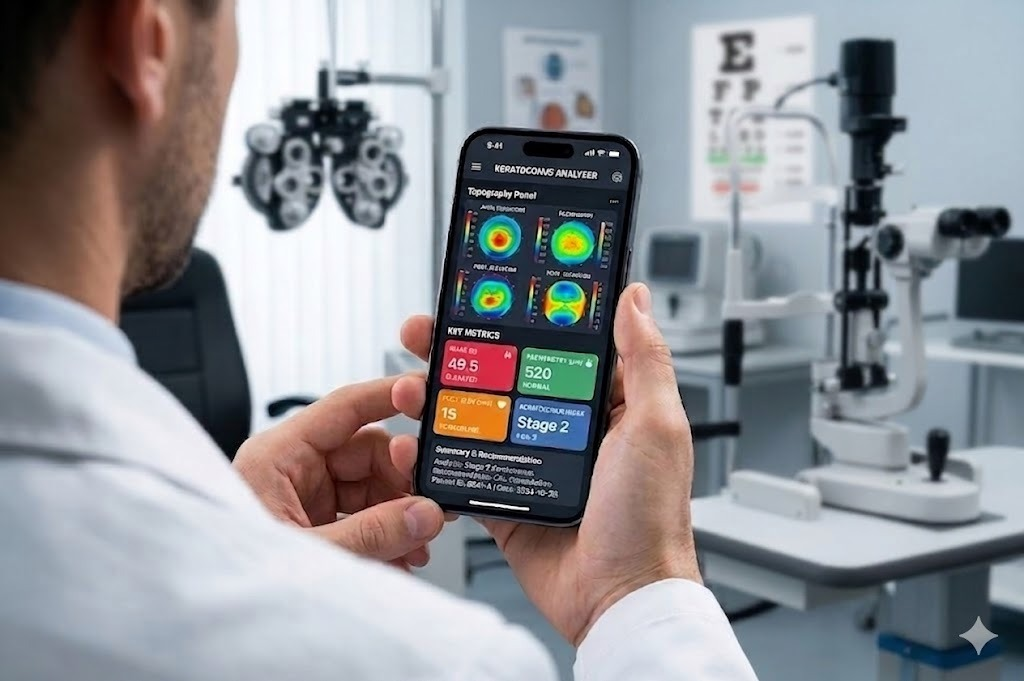
\includegraphics[width=0.5\linewidth]{img/humo.jpeg}
            \caption{Representación visual de la aplicación.}
        \end{figure}

    \phantomsection
    \subsection{Descripción de los usuarios y usos posibles}
    
        \subsubsection*{Usuarios}
    
            Los usuarios destinatarios corresponderían a los médicos oftalmólogos generales, especialistas en córnea y técnicos en centros de optometría de alta complejidad, los cuales dispongan del equipo necesario para la realización de los estudios.
    
        \subsubsection*{Usos posibles}
    
            \begin{itemize}
                \item Detección temprana de queratocono subclínico en pacientes jóvenes.
                
                \item Estandarización de criterios diagnósticos en la interpretación de mapas corneales.
            \end{itemize}

        \subsection{Análisis de demanda}
        
            Aunque no se manifieste una demanda excesiva de una herramienta de soporte a la decisión por parte de los profesionales, existe una necesidad creciente por la misma, resultante de la naturaleza subjetiva de los análisis  de los estudios. Estos son dependientes de la experiencia de los oftalmólogos, lo cual aumenta la probabilidad de cometer errores en la detección, sobre todo en etapas subclínicas, es decir, etapas iniciales donde la manifestación suele confundirse con enfermedades más comunes y menos nocivas~\cite{deteccion_temprana}. 
            
            En este apartado el producto ofrece la capacidad de mitigar dicha subjetividad al actuar como una ``segunda opinión experta'', reduciendo la dependencia de la experiencia del médico de turno, garantizando un diagnóstico preciso y estandarizado independientemente de quién evalúe el estudio.
            
            Esto descentralizaría, en cierta medida, la atención médica de alta complejidad, un factor especialmente crítico en provincias o zonas alejadas de las grandes capitales generando interés enorme para centros médicos regionales derivando a los centros de alta complejidad únicamente los casos que realmente lo requieren. 
            
            La demanda se sustenta en:
            
            \begin{itemize}
                \item La necesidad de reducir el margen de error diagnóstico~\cite{deteccion_temprana}.
                
                \item El alto volumen en Misiones de afectados que requieren el diagnóstico preciso de la patología~\cite{misiones}.  
                
                \item El respaldo de normativas para la modernización tecnológica en salud pública y privada~\cite{dispo_2318,dispo_9688}.
            \end{itemize}

        \phantomsection
        \subsection{Análisis de la oferta}

            El mercado global está dominado por un grupo reducido de empresas que comercializan sistemas cerrados, los cuales analizan y reestructuran los datos provenientes de los mismos equipos sin realizar predicciones ni diagnósticos sobre los mismos, donde el software de análisis depende obligatoriamente de tener sus dispositivos propietarios. A nivel nacional, no existen competidores directos con un software como producto médico específico para queratocono. La Tabla~\ref{tabla:oferta_cualitativa} resume las características cualitativas de los competidores identificados.

            \begingroup \setstretch{1.1}
            \begin{longtblr}[
                caption = Características cualitativas de la oferta competitiva,
                label = tabla:oferta_cualitativa
                ]{
                    colspec = {Q[l,m,3.5cm] X[l,m] X[l,m]},
                    cells = {font=\small},
                    row{1} = {bg=gray!15, font=\small\bfseries, halign=c},
                    hlines, vlines,
                    rowsep = 3pt, colsep = 5pt
                }
                
                Competidor & Descripción & Limitación \\
                
                Oculus (Familia Pentacam) 
                & Referente del sector. Oferta desde modelos básicos hasta el Pentacam AXL Wave con biometría y wavefront~\cite{oculus}. 
                & Sistema cerrado. Software dependiente de hardware propietario. \\

                Topcon Healthcare 
                & Conectividad mediante Harmony e IDHea. Integra datos de topógrafos de Placido (CA-800) para análisis longitudinal asistido por IA~\cite{topcon}. 
                & Sistema cerrado. Sin módulo específico para queratocono. \\

                KERAFound (Dr. Shafi Balal / Moorfields) 
                & Plugin de código abierto en desarrollo para predecir riesgo de progresión del queratocono~\cite{shafi_balal}. 
                & En fase de investigación. Sin integración a sistemas médicos. \\

                KeratoDetect 
                & Algoritmo CNN para detección binaria subclínica~\cite{kerato_detect}. 
                & Código cerrado. Solo detección, sin estratificación ni integración. \\

                AEYE 
                & Sistema multi-agente de IA para detección de queratocono y evaluación de elegibilidad refractiva~\cite{aeye}. 
                & Diseñado para sistemas internacionales de alta gama. \\

                Entelai 
                & Startup Argentina para análisis de imágenes médicas con IA~\cite{entelai}. 
                & Solución general. Sin módulo específico para queratocono. \\

                \textbf{Nuestro proyecto} 
                & Software independiente (SaMD) multimodal. Detección temprana con explicación visual en una aplicación web accesible.
                & Desarrollo acotado a normativas ANMAT. Necesidad de validación local. \\
                
            \end{longtblr}
            \endgroup

        \phantomsection
        \subsection{Análisis de precios}

            La Tabla~\ref{tabla:precios_cuantitativa} presenta la comparativa de precios y costos de los competidores identificados, diferenciando entre inversión inicial, modelo de facturación y costo por uso.

            \begingroup \setstretch{1.1}
            \begin{longtblr}[
                caption = Comparativa de precios y costos de la oferta competitiva,
                label = tabla:precios_cuantitativa
                ]{
                    colspec = {Q[l,m,4cm] X[l,m] X[l,m]},
                    cells = {font=\small},
                    row{1} = {bg=gray!15, font=\small\bfseries, halign=c},
                    hlines, vlines,
                    rowsep = 3pt, colsep = 5pt
                }
                
                Competidor & Inversión inicial & Modelo de facturación \\
                
                Sistemas tradicionales (Oculus/Ziemer) 
                & USD \$\,20.000 a USD \$\,40.000 por equipo + software 
                & Licencia cerrada e inflexible \\

                Referente IA local (Entelai) 
                & No requiere hardware propio 
                & SaaS / Pay-per-scan: $\approx$\,\$\,3.790 + IVA por informe~\cite{entelai} \\

                \textbf{Nuestra propuesta} 
                & No requiere hardware nuevo. Procesa los mapas que exportan los equipos existentes (en el prototipo, Orbscan)
                & Suscripción mensual SaaS \\
                
            \end{longtblr}
            \endgroup

            \subsubsection*{Estructura de costos del proyecto}
            
            \begin{itemize}[leftmargin=*]
                \item \textbf{Infraestructura mensual:} Aproximadamente \$\,41.600 ARS. Esto incluye el servidor VPS (KVM 4 de Hostinger a $\approx$\,\$\,23.300) y la plataforma de entrenamiento (Google Colab Pro a $\approx$\,\$\,18.300 con impuestos incluidos).  
    
                \item \textbf{Validación médica:} El costo operativo de un especialista para auditoría de datos es de $\approx$\,\$\,30.000 ARS por hora.  
    
                \item \textbf{Barrera regulatoria (ANMAT):} El registro del producto Clase II cuesta \$\,52.000 ARS, pero la habilitación inicial de la empresa como fabricante/importador requiere un pago único de \$\,1.523.100 ARS.
            \end{itemize}

        \phantomsection
        \subsection{Análisis de la comercialización}
        
            \subsubsection{Definición del producto requerido por los consumidores potenciales}
        
            Los oftalmólogos ``demandan'' una herramienta que sea:
        
            \begin{itemize}
                \item \textbf{Interoperable:} Capaz de recibir imágenes de distintos dispositivos diagnósticos.  
        
                \item \textbf{Intuitiva:} Con una interfaz amigable (React) que no requiera conocimientos técnicos en IA.  
        
                \item \textbf{Fiable:} Que proporcione evidencia visual (XAI) para sustentar la decisión clínica ante el paciente.
            \end{itemize}
        
            \subsubsection{Estrategia de comunicación de los consumidores potenciales}
        
            La estrategia de comunicación para incentivar la adopción por parte de los consumidores potenciales (clínicas, centros de salud y oftalmólogos) se estructurará en los siguientes focos:
        
            \begin{itemize}
                 \item \textbf{Mensaje central y propuesta de valor:} Difusión de los beneficios clave del sistema (estandarización clínica y optimización de recursos), posicionándolo como una ``segunda opinión'' que reduce la subjetividad en análisis topográficos y tomográficos, previniendo errores en etapas subclínicas.  
            
                \item \textbf{Difusión científica:} Publicación de resultados de la validación con datos locales en congresos regionales o internacionales de oftalmología o informática.  
        
                \item \textbf{Marketing directo:} Presentaciones institucionales en clínicas privadas de Misiones, el Ministerio de Salud Pública o interesados.  
        
                \item \textbf{Presencia digital y educativa:} Difusión en redes profesionales (LinkedIn), envío de newsletters especializados del sector salud y organización de webinars técnicos para la adopción y actualización continua de los profesionales.
            \end{itemize}
        
            \subsubsection{Estrategia de venta y distribución del producto}
        
                La estrategia de venta y distribución para el software se centra en un modelo de servicio digital escalable, diseñado para integrarse de manera directa en el flujo de trabajo actual del oftalmólogo. El objetivo es facilitar el acceso al soporte diagnóstico mediante una infraestructura en la nube práctica, rápida y eficaz, planteando a la herramienta como un complemento para el equipamiento diagnóstico tradicional.

            \vspace{-0.5 cm}
            \paragraph{Distribución y acceso:}
            
            \begin{itemize}
                \item El software se desplegará en un servidor VPS.
                
                \item El acceso al usuario final se realiza mediante una aplicación web, bajo un modelo de suscripción, que permite al oftalmólogo consultar los resultados desde el navegador de cualquier dispositivo.
            \end{itemize}

            \vspace{-0.5 cm}
            \paragraph{Canales de venta:}
            
            \begin{itemize}
                \item Venta directa a instituciones de salud.  
                
                \item Colaboración con distribuidores de equipamiento oftalmológico para ofrecer el software como un valor agregado (plugin) a sus equipos.  
                
                \item Asistencia técnica remota para garantizar el mantenimiento y actualización del sistema.
            \end{itemize}

        \phantomsection
        \subsection{Estudio de factibilidad y viabilidad del proyecto}
        
            \subsubsection*{Criterios de ponderación}
        
            \paragraph{Viabilidad técnica} (40\,\% de influencia) Determina si el equipo de desarrollo cuenta con los recursos y experiencia para cumplir los requisitos.
        
            \begin{itemize}
                \item \textbf{Accesibilidad de tecnologías y datos:} Evaluar la facilidad para obtener \textit{hardware} de entrenamiento, herramientas de \textit{software} y el acceso a los datasets multimodales.
        
                \item \textbf{Capacidad técnica del equipo:} Medir si los integrantes poseen las habilidades necesarias en \textit{Deep Learning}, desarrollo \textit{backend/frontend} y manejo de normativas médicas.
        
                \item \textbf{Interoperabilidad:} Capacidad del sistema para integrarse con diferentes equipos de diagnóstico (por ejemplo, Orbscan, Pentacam o Sirius).
        
                \item \textbf{Mantenibilidad del sistema:} La facilidad con la que el software puede ser actualizado, corregido o adaptado a nuevas versiones o cambios en los formatos de salida de los equipos de diagnóstico.
            \end{itemize}
        
            \paragraph{Viabilidad jurídica} (25\,\% de influencia) Para asegurar el cumplimiento normativo respecto a la salud.
        
            \begin{itemize}
                \item \textbf{Cumplimiento de normativas ANMAT:} Factibilidad de registrar el software como producto médico (SaMD) bajo las disposiciones N.º 2318/2002~\cite{dispo_2318} y N.º 9688/2019~\cite{dispo_9688}, clasificándolo como Clase II.  
                
                \item \textbf{Protección de datos personales:} Garantizar que los procesos de anonimización de datos locales cumplan con la Ley N.º 25.326 (2000) de Protección de los Datos Personales~\cite{ley_25326}.  
                
                \item \textbf{Consentimiento informado:} Viabilidad de gestionar los permisos legales necesarios con los pacientes de Misiones para el uso de sus muestras en la validación.
            \end{itemize}

            \vspace{-0.5 cm}
            \paragraph{Viabilidad operativa} (20\,\% de influencia) Analizar si el sistema se utilizará y funcionará al instalarse.
        
            \begin{itemize}
                \item \textbf{Predisposición y aceptación del usuario:} Nivel de apertura de los oftalmólogos para adoptar herramientas de IA como apoyo diagnóstico.  
                
                \item \textbf{Facilidad de uso e interfaz:} Evaluación de si la curva de aprendizaje de la aplicación es lo suficientemente baja para el personal médico con poca experiencia en el uso de herramientas digitales.  
                
                \item \textbf{Integración al flujo de trabajo:} Determinar si el sistema agiliza o entorpece la consulta diaria del especialista. 
            \end{itemize}

            \vspace{-0.5 cm}
            \paragraph{Viabilidad económica} (15\,\% de influencia) Evalúa la rentabilidad y la capacidad de solventar los gastos.
        
            \begin{itemize}
                \item \textbf{Costos directos de desarrollo e implementación:} Incluye licencias de plataformas de desarrollo (Colab Pro por ejemplo), \textit{hosting} VPS y los aranceles de ANMAT.  
                
                \item \textbf{Costos de validación clínica:} Honorarios de los especialistas médicos por las horas dedicadas a auditar el sistema o consultas pertinentes.  
                
                \item \textbf{Relación costo-beneficio:} Compara el esfuerzo económico invertido frente al valor o ahorro que el proyecto generará a largo plazo a los especialistas.
            \end{itemize}
        
            \subsubsection*{Análisis por criterio}

            \paragraph{Viabilidad técnica}

            \begin{itemize}
                \item \textbf{Accesibilidad de tecnologías y datos:} Para el entrenamiento se dispone del \textit{dataset} público y multimodal CornOrb~\cite{zenodo}, cuyo análisis exploratorio confirmó que es adecuado como punto de partida (ver capítulo Desarrollo). Las herramientas de desarrollo son de uso libre (Python, FastAPI, React) y la capacidad de cómputo necesaria se obtiene mediante Google Colab Pro. Las muestras locales se encuentran en proceso de solicitud a nueve centros de salud y profesionales; su obtención no condiciona el desarrollo del prototipo.

                \item \textbf{Capacidad técnica del equipo:} Los integrantes cuentan con experiencia previa, en el ámbito académico, en el desarrollo de modelos de aprendizaje profundo y de aplicaciones web. El conocimiento normativo se complementa con el asesoramiento del abogado consultor previsto en el presupuesto.

                \item \textbf{Interoperabilidad:} Es el aspecto más limitado. El prototipo procesa únicamente los mapas corneales de equipos Orbscan, tal como los provee CornOrb. La compatibilidad con otros equipos, como Pentacam o Sirius, depende de acceder a sus archivos de exportación y se plantea como trabajo futuro.

                \item \textbf{Mantenibilidad del sistema:} La separación del sistema en módulos independientes (preprocesamiento, modelo, API e interfaz) y su encapsulamiento mediante contenedores permiten actualizar cada parte por separado. Un cambio en el formato de exportación de un equipo, por ejemplo, solo afecta al módulo de preprocesamiento.
            \end{itemize}

            \paragraph{Viabilidad jurídica}

            \begin{itemize}
                \item \textbf{Cumplimiento de normativas ANMAT:} El sistema se categoriza como producto médico Clase II, cuya inscripción exige demostrar su seguridad y eficacia mediante validación clínica. Este requisito corresponde a la proyección del producto (cuarta fase), mientras que el prototipo del PFI no se utiliza para tomar decisiones clínicas. Desde el inicio se lleva la documentación y trazabilidad que la inscripción requerirá.

                \item \textbf{Protección de datos personales:} La Ley N.º 25.326 (2000) considera a los datos referidos a la salud como datos sensibles, que cuentan con el mayor nivel de protección~\cite{ley_25326}. Por ello, todo estudio utilizado debe estar anonimizado: los de CornOrb ya lo están, y las muestras locales deberán anonimizarse en su origen, antes de ser compartidas con el equipo.

                \item \textbf{Consentimiento informado:} El uso de estudios de pacientes locales requiere contar con su consentimiento. Su gestión depende de los centros colaboradores y forma parte de las solicitudes en curso.
            \end{itemize}

            \paragraph{Viabilidad operativa}

            \begin{itemize}
                \item \textbf{Predisposición y aceptación del usuario:} Se estima favorable, dado que la herramienta responde a una dificultad diagnóstica reconocida (ver Análisis del problema) y se presenta como apoyo al especialista y no como reemplazo. Aun así, la resistencia a adoptar herramientas de IA es un riesgo identificado (R7), por lo que la aceptación deberá confirmarse en las pruebas con usuarios.

                \item \textbf{Facilidad de uso e interfaz:} Al tratarse de una aplicación web, no requiere instalación y puede utilizarse desde el navegador de cualquier dispositivo. El informe presenta el resultado, su nivel de confianza y el mapa de calor que lo justifica, y el diseño de la interfaz cuenta con un especialista en experiencia de usuario.

                \item \textbf{Integración al flujo de trabajo:} El oftalmólogo carga los mapas que ya exporta su equipo, sin modificar la forma en que se realiza el estudio. El sistema agrega un paso a la consulta, cuyo impacto en el tiempo de atención deberá evaluarse en las pruebas de usabilidad.
            \end{itemize}

            \paragraph{Viabilidad económica}

            \begin{itemize}
                \item \textbf{Costos directos de desarrollo e implementación:} La infraestructura tecnológica tiene un costo mensual acotado (servidor VPS, Google Colab Pro y herramientas de desarrollo). Los gastos de mayor peso corresponden a la habilitación de la empresa ante la ANMAT y a los recursos humanos (ver sección Presupuesto).

                \item \textbf{Costos de validación clínica:} Los honorarios del oftalmólogo consultor representan el ítem más costoso del presupuesto, y se concentran en la validación clínica de la proyección del producto.

                \item \textbf{Relación costo-beneficio:} Frente al costo de un estudio topográfico, los tratamientos de las etapas avanzadas de la enfermedad son entre veinte y más de sesenta veces más caros (ver Impacto económico), por lo que una detección temprana representa un ahorro potencial considerable. Para el proyecto, la viabilidad depende de financiar la inversión inicial hasta que el modelo de suscripción genere ingresos, lo que se aborda mediante el préstamo descrito en la sección Distribución financiera.
            \end{itemize}

            La Tabla~\ref{tabla:viabilidad} resume la evaluación de cada criterio según su ponderación.

            \begingroup \setstretch{1.1}
            \begin{longtblr}[
                caption = Resumen de la evaluación de viabilidad del proyecto,
                label = tabla:viabilidad
                ]{
                    colspec = {Q[l,m,2.6cm] Q[c,m,1.6cm] Q[c,m,2.2cm] X[l,m]},
                    cells = {font=\small},
                    row{1} = {bg=gray!15, font=\small\bfseries, halign=c},
                    hlines, vlines,
                    rowsep = 3pt, colsep = 5pt
                }

                Criterio & Peso & Evaluación & Principal condicionante \\

                Técnica & 40\,\% & Alta & Compatibilidad limitada a equipos Orbscan en el prototipo \\

                Jurídica & 25\,\% & Media & La inscripción ante la ANMAT requiere validación clínica \\

                Operativa & 20\,\% & Favorable & Aceptación a confirmar en pruebas con usuarios \\

                Económica & 15\,\% & Media & Financiamiento de la inversión inicial hasta el lanzamiento \\

            \end{longtblr}
            \endgroup

            El criterio de mayor peso, la viabilidad técnica, es también el más favorable, lo que respalda la factibilidad del prototipo planteado para el PFI. Los condicionantes jurídicos y económicos recaen principalmente sobre la proyección del producto, y se encuentran contemplados en la planificación y en la gestión de riesgos.

    \vspace{-0.5 cm}
    \phantomsection
    \section{Presupuesto}

        \phantomsection
        \subsection{Recursos materiales}

            Al tratarse de un software como producto médico, los insumos requeridos son exclusivamente digitales. Afortunadamente, se obtendrán a través de vías institucionales o de código abierto, por lo que no representan un costo económico:

            \begin{itemize}
                \item \textbf{Muestras locales:} Lote de 150 imágenes de topografías corneales anonimizadas, provistas por el consultorio médico asociado para realizar la validación clínica local de los algoritmos.
    
                \item \textbf{Datasets de información:} Bases de datos públicas e internacionales con casos de queratocono, las cuales se utilizarán en la etapa de entrenamiento inicial de la Inteligencia Artificial.
            \end{itemize}

            \begin{itemize}
                \item \textbf{Computadoras portátiles (\textit{Notebooks}):} Se requiere \textit{hardware} estándar para las tareas de programación y desarrollo local durante la ejecución del proyecto, así como para eventuales ajustes o mantenimientos futuros. Tomando como referencia equipos con procesador Intel Core i7 y 16 GB de RAM, el valor de mercado actual ronda entre los \$\,1.800.000 y \$\,2.100.000 ARS por unidad. Teniendo en cuenta que se planea adquirir estos equipo para el desarrollo exclusivo de este proyecto, uno por cada integrante, el costo total estimado es de \$\,4.200.000.
            \end{itemize}

        \phantomsection
        \subsection{Recursos humanos}

            El desarrollo del proyecto será llevado a cabo tanto por mano de recursos humanos propios, como también por parte de personal adicional o externo para las áreas de marketing y diseño. La estructura de los recursos humanos es la siguiente:
    
            \subsubsection*{Recursos humanos propios}
    
                Los valores calculados a continuación se basan en los honorarios recomendados por el Consejo Profesional de Ciencias Informáticas de Córdoba \cite{honorarios_profesionales_cordoba}. Sin embargo, para garantizar la viabilidad del proyecto, se asignaron retribuciones simbólicas basadas en el valor de un salario Mínimo Vital y Móvil (SMVM) \cite{cita:SMVM} en proporción a una jornada laboral de cuatro horas diarias.
                
                \begin{itemize}
                    \item \textbf{Programador Inteligencia Artificial:} Este rol es el principal encargado del desarrollo y entrenamiento del modelo en la primera fase del proyecto. Con una participación de 9 meses y dedicación del 50\,\%, el costo total, basado en su retribución simbólica, estimado es de \$\,3.171.600.
        
                    \item \textbf{Desarrollador Web Full Stack:} Este rol comienza a desarrollarse en la segunda fase del proyecto, correspondiente a la implementación e integración. Se encargará del desarrollo del \textit{backend} y \textit{frontend} de la aplicación. Con una participación de 2 meses y dedicación del 50\,\% el costo total, basado en su retribución simbólica, estimado es de \$\,704.800.
                \end{itemize}
    
            \subsubsection*{Recursos humanos adicionales}
                
                Los valores calculados a continuación se basan en el salario mediano de dichos roles~\cite{cita:salario_marketing,cita:salario_UX_UI}.
                
                \begin{itemize}
                    \item \textbf{Diseñador UX y UI:} Su actividad se centrará en la segunda fase, de implementación e integración junto a los desarrolladores web, diseñando interfaces intuitivas y amigables para que sea simple de usar para usuarios no técnicos. Con una participación de 1 mes y una dedicación del 30\,\% el costo total estimado es de \$\,480.000.
        
                    \item \textbf{Especialista en marketing digital:} Este perfil se enfocará en la creación de campañas de marketing digital y en realizar sugerencias  en cuanto a la información presentada en \textit{newsletters}, \textit{webinars} y congresos científicos. Con una participación de 1 mes y una dedicación del 20\,\% el costo total estimado es de \$\,162.000.
                \end{itemize}

            \vspace{-0.25 cm}
            \begingroup \setstretch{1.1}
            \begin{longtblr}[
                caption = Recursos humanos propios que intervendrán en el proyecto,
                label = tabla:rrhh_propios
                ]{
                    colspec = {X[l,m] Q[c,m,1cm] Q[r,m,2.3cm] Q[r,m,2.1cm] Q[c,m,1.4cm] Q[c,m,1.2cm] Q[r,m,2.3cm]},
                    cells = {font=\footnotesize},
                    row{1} = {bg=gray!15, font=\footnotesize\bfseries, halign=c},
                    row{4} = {bg=gray!15, font=\footnotesize\bfseries},
                    hlines, vlines,
                    rowsep = 3pt, colsep = 3pt
                }
            
                Profesión / función en el proyecto & Cant. & Costo mensual real c/u & Retribución simbólica & Meses de partic. & \% de dedic. & Costo total \\
            
                Programador IA & 2 & \$\,3.783.577,52 & \$\,352.400,00 & 9 & 50 & \$\,3.171.600,00 \\
            
                Desarrollador Web Full Stack & 2 & \$\,3.453.169,23 & \$\,352.400,00 & 2 & 50 & \$\,704.800,00 \\
            
                \SetCell[c=6]{r} TOTAL & & & & & & \$\,3.876.400,00 \\
            
            \end{longtblr}
            \endgroup

            \vspace{-0.75 cm}
            \begingroup \setstretch{1.1}
            \begin{longtblr}[
                caption = Recursos humanos adicionales requeridos en el proyecto,
                label = tabla:rrhh_adicionales
                ]{
                    colspec = {Q[l,m,2.4cm] X[l,m] Q[r,m,2.5cm] Q[c,m,1.5cm] Q[c,m,1.4cm] Q[r,m,2.3cm]},
                    cells = {font=\small},
                    row{1} = {bg=gray!15, font=\small\bfseries, halign=c},
                    row{4,5} = {bg=gray!15, font=\small\bfseries},
                    hlines, vlines,
                    rowsep = 3pt, colsep = 5pt
                }
            
                Profesión u oficio & Función en el proyecto & Costo total mensual & Meses de partic. & \% de dedic. & Costo total \\
            
                Diseñador web & Diseño de las interfaces UI/UX & \$\,1.600.000,00 & 1 & 30 & \$\,480.000,00 \\
            
                Idóneo & Marketing digital & \$\,810.000,00 & 1 & 20 & \$\,162.000,00 \\
            
                \SetCell[c=5]{r} TOTAL & & & & & \$\,642.000,00 \\
            
                \SetCell[c=5]{r} TOTAL DE RECURSOS HUMANOS & & & & & \$\,4.518.400,00 \\
            
            \end{longtblr}
            \endgroup

        \phantomsection
        \subsection{Recursos económicos}
    
            Esta sección engloba la auditoría médica por parte del oftalmólogo, consultas legales con un abogado, la infraestructura en la nube y los servicios necesarios para el desarrollo del producto.
    
            \begin{itemize}
                \vspace{0.25 cm}
                \item \textbf{Licenciado en Oftalmología - Consultor:} Se tomará como referencia el valor de hora médica definida por el colegio de médicos de la provincia de Misiones \cite{cita:honorario_oftalmólogo}, con un costo de \$\,129.000 ARS por hora médica y un tiempo de estimado de 40 horas, distribuidas a lo largo de aproximadamente 2 meses. Se elige este valor, ya que, para fines de este proyecto, no se realizarán consultas clínicas de rutina, sino que se realizará tareas de alta complejidad fuera del consultorio, como por ejemplo validación de datos y pruebas de experiencia de usuario. 
    
                \item \textbf{Abogado - Consultor:} Ayudará en el asesoramiento legal en cuanto a encuadre regulatorio ante la ANMAT, redacción de términos y condiciones de uso del software y registro de propiedad intelectual. Basándonos en los valores establecidos por el colegio de abogados de la provincia de Misiones \cite{cita:honorario_abogado} el costo total estimado es de \$\,387.640, teniendo el valor de un salario Mínimo Vital y Móvil (SMVM) \cite{cita:SMVM}, cuatro consultas formales de un valor de 20\,\% de un SMVM y la redacción de documentos por el valor del 30\,\% de un SMVM.
    
                \item \textbf{Google Colaboratory (Pro):} Entorno \textit{Cloud} con acceso a GPU para el entrenamiento de los modelos de IA. Su costo de suscripción es de aproximadamente \$\,18.300 ARS mensuales (\$\,10 USD + impuesto país).
    
                \item \textbf{Suscripción a \textit{Claude Code}:} herramienta para acelerar el desarrollo del sistema de análisis de topografías corneales mediante la automatización de la escritura, refactorización y depuración del código. Dicha suscripción tiene un valor de aproximadamente \$\,31.000 (\$\,20 USD + impuesto país) por mes.
    
                \item \textbf{Servidor VPS:} Infraestructura virtual para el despliegue de la API \textit{backend} y el \textit{frontend}. Su costo ronda los \$\,41.600 ARS mensuales.
            \end{itemize}
            
            \begingroup \setstretch{1.1}
            \begin{longtblr}[
                caption = Consultoría y servicios tecnológicos a contratar,
                label = tabla:consultoria_servicios
                ]{
                    colspec = {X[l,m] Q[r,m,2.8cm] Q[c,m,2.6cm] Q[r,m,2.8cm]},
                    cells = {font=\small},
                    row{1} = {bg=gray!15, font=\small\bfseries, halign=c},
                    row{7} = {bg=gray!15, font=\small\bfseries},
                    hlines, vlines,
                    rowsep = 3pt, colsep = 5pt
                }
            
                Descripción & Costo mensual & Meses de partic. & Costo total \\
            
                Google Colaboratory & \$\,18.300,00 & 12 & \$\,219.600,00 \\
            
                Suscripción Claude Code & \$\,31.000,00 & 12 & \$\,372.000,00 \\
            
                VPS & \$\,41.600,00 & 6 & \$\,249.600,00 \\
            
                Abogado - Consultor & \$\,96.910,00 & 4 & \$\,387.640,00 \\
            
                Lic. Oftalmología - Consultor & \$\,1.720.000,00 & 3 & \$\,5.160.000,00 \\
            
                \SetCell[c=3]{r} TOTAL & & & \$\,6.388.840,00 \\
            
            \end{longtblr}
            \endgroup

            Comprende la logística y movilidad física para las reuniones con el oftalmólogo colaborador, pago de la inscripción del software como producto médico, autorización de la empresa fabricante frente a la ANMAT y costos pertinentes para la divulgación del producto en el congreso nacional de oftalmología.
    
            \begin{itemize}
                \item \textbf{Traslado desarrolladores hacia clínica de oftalmólogo colaborador (Oberá - Alem):} Considerando el viaje en colectivo, el costo aproximado es de \$\,5.000 ARS por viaje, dependiendo de la empresa. Teniendo en cuenta dos viajes, considerando viaje de ida y regreso, da un total de \$\,20.000.
    
                \item \textbf{Registro del producto ante la ANMAT:} Se registrará el software como producto médico Clase II ante la ANMAT; este registro es un pago único de \$\,52.000 ARS.
    
                \item \textbf{Autorización de funcionamiento de empresa fabricante de productos médicos frente a la ANMAT:} Puesto que, las actividades de fabricación o importación de productos médicos, solo pueden efectuarse si se cuenta con esta autorización previa, siendo un pago único de \$\,1.523.100.
    
                \item \textbf{Traslado de desarrolladores al congreso nacional de oftalmología (Oberá - Buenos Aires):} Considerando el boleto de colectivo de larga distancia y traslado urbano, el costo aproximado es de \$\,85.000 ARS por viaje, dependiendo de la empresa de transporte. Teniendo en cuenta dos viajes, considerando viaje de ida y regreso, da un subtotal de \$\,340.000 y teniendo en cuenta un rango de \$\,160.000 de costos de transporte urbano y viáticos el total alcanzaría los \$\,500.000.
    
                \item \textbf{Inscripción al congreso nacional de oftalmología:} Dado que, el Congreso Nacional de Oftalmología (CNO) es el principal encuentro científico y académico para médicos oftalmólogos y profesionales de la salud visual a nivel nacional, se considera pertinente su inscripción al mismo. Para personas técnicas que presenten una carta de recomendación de un oftalmólogo matriculado, el costo es de \$\,24.000 aproximadamente.
            \end{itemize}

            \begingroup \setstretch{1.1}
            \begin{longtblr}[
                caption = {Costos de movilidad, logística, inscripción a congresos y matriculación},
                label = tabla:otros_costos
                ]{
                    colspec = {X[l,m] Q[r,m,3cm]},
                    cells = {font=\small},
                    row{1} = {bg=gray!15, font=\small\bfseries, halign=c},
                    row{7} = {bg=gray!15, font=\small\bfseries},
                    hlines, vlines,
                    rowsep = 3pt, colsep = 5pt
                }
            
                Descripción & Costo total \\
            
                Traslado (4) desarrolladores hacia clínica de oftalmólogo colaborador (Oberá / Leandro N. Alem) & \$\,20.000,00 \\
            
                Registro de producto médico Clase II - ANMAT & \$\,52.000,00 \\
            
                Autorización de funcionamiento de empresa fabricante de productos médicos frente a la ANMAT & \$\,1.523.100,00 \\
            
                Traslado (4) al congreso nacional de oftalmología (Oberá / Buenos Aires) & \$\,500.000,00 \\
            
                Inscripción a congreso nacional de oftalmología & \$\,24.000,00 \\
            
                \SetCell[c=1]{r} TOTAL & \$\,2.119.100,00 \\
            
            \end{longtblr}
            \endgroup

        \vspace{-0.5 cm}
        \phantomsection
        \subsection{Distribución financiera}
        \label{sec:distribucion_financiera}
        
            Durante el análisis financiero realizado, se identifica una fuerte inversión inicial seguida de una escalabilidad comercial basada en un modelo de suscripción (SaaS). Cabe aclarar que el desarrollo del proyecto se elabora en el ámbito de la Facultad de Ingeniería de Oberá (UNaM), lo que permite prescindir de costos de infraestructura como alquiler, servicios básicos y equipamiento de espacio de trabajo. Estos se encuentran cubiertos por la institución. Durante los primeros 10 meses del proyecto, el flujo de caja operativo es estrictamente negativo, puesto que al no existir un producto comercializable aún, no se registran ingresos por ventas.

            Para asegurar la viabilidad del proyecto durante su fase inicial, se apalanca el flujo de caja con un préstamo estratégico de \$\,20.000.000 ARS del Fondo de Crédito Misiones, el cual cuenta con una tasa subsidiada (TNA del 28\,\%) y 6 meses de gracia para el pago de capital.
        
            A partir del mes 11, el sistema se lanza comercialmente con un modelo de suscripción accesible de \$\,150.000 mensuales, logrando la adhesión del oftalmólogo colaborador como primer suscriptor. Durante los primeros tres años, la estrategia de captación se enfoca en sumar progresivamente de 2 a 3 clínicas cabecera, equipadas con tomógrafos corneales, dentro de las principales urbes de Misiones, como Posadas, Oberá y Eldorado.
            
            Finalmente, entre el cuarto y el sexto año, la proyección financiera escala de manera conservadora hasta alcanzar un máximo de 9 suscripciones activas, dejando vía libre hacia un crecimiento a nivel nacional.

        \phantomsection
        \subsection{Flujo de caja}

            Las Figuras~\ref{fig:flujo_meses} y~\ref{fig:flujo_anios} muestran la evolución del flujo de caja durante los primeros doce meses y los primeros seis años del proyecto, respectivamente. El detalle de los ingresos y egresos que los componen se presenta en las Figuras~\ref{fig:anexo_caja_desarrollo} y~\ref{fig:anexo_caja_años} del Anexo.

            \begin{figure}[tbp]
                \centering
                \makebox[\linewidth][c]{\hspace*{1 cm}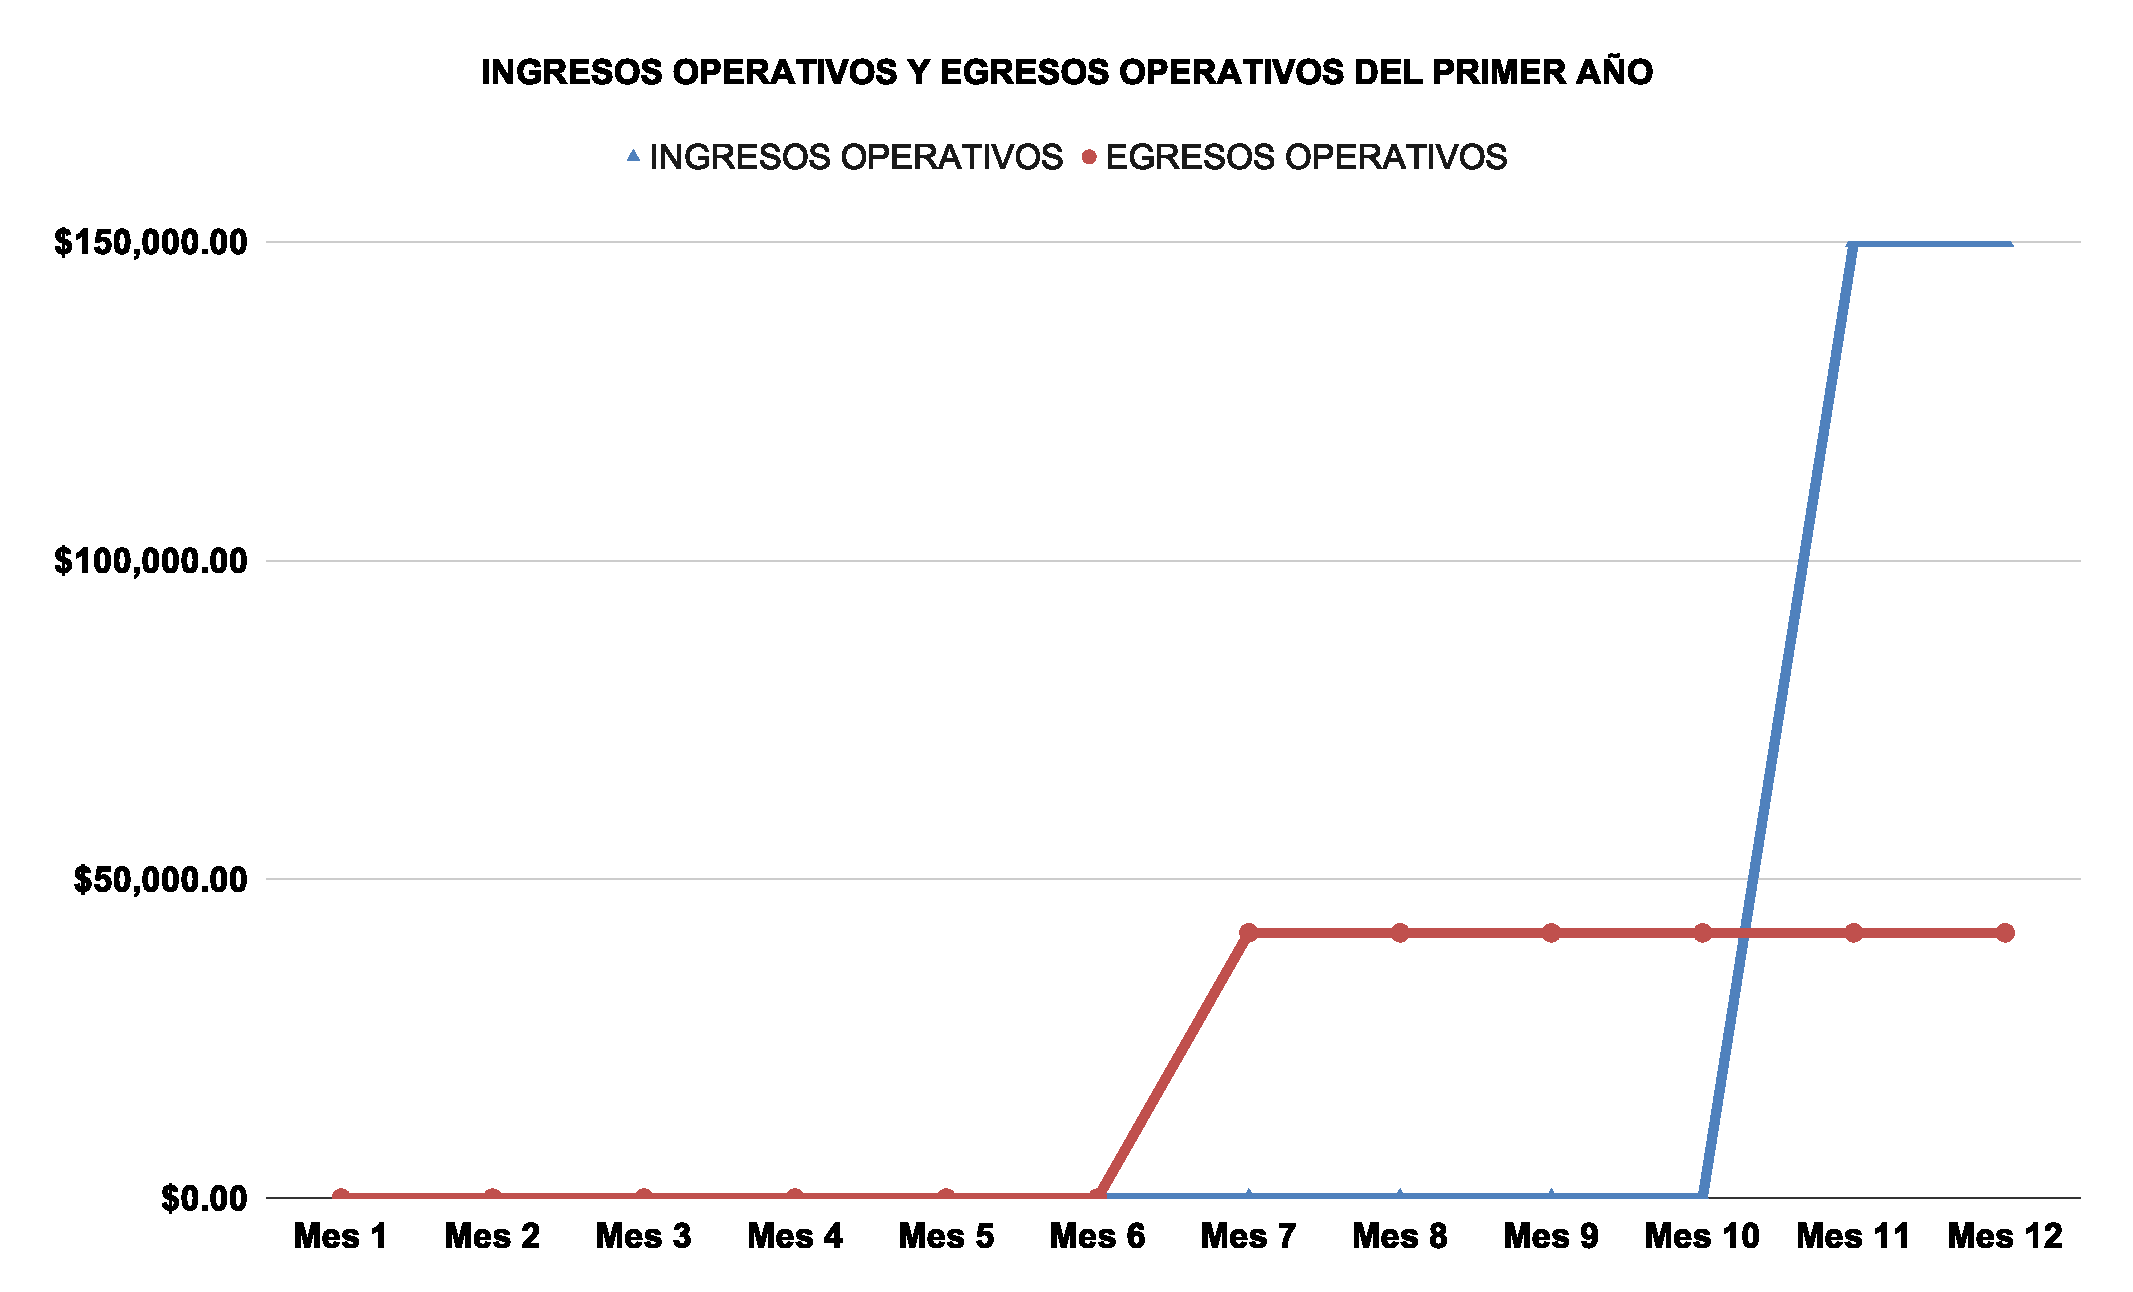
\includegraphics[height=0.28\textheight]{img/flujo_meses_grafico.pdf}}
                \caption{Gráfico de flujo de caja correspondiente a los primeros doce meses.}
                \label{fig:flujo_meses}
            \end{figure}

            \begin{figure}[tbp]
                \centering
                \makebox[\linewidth][c]{\hspace*{1 cm}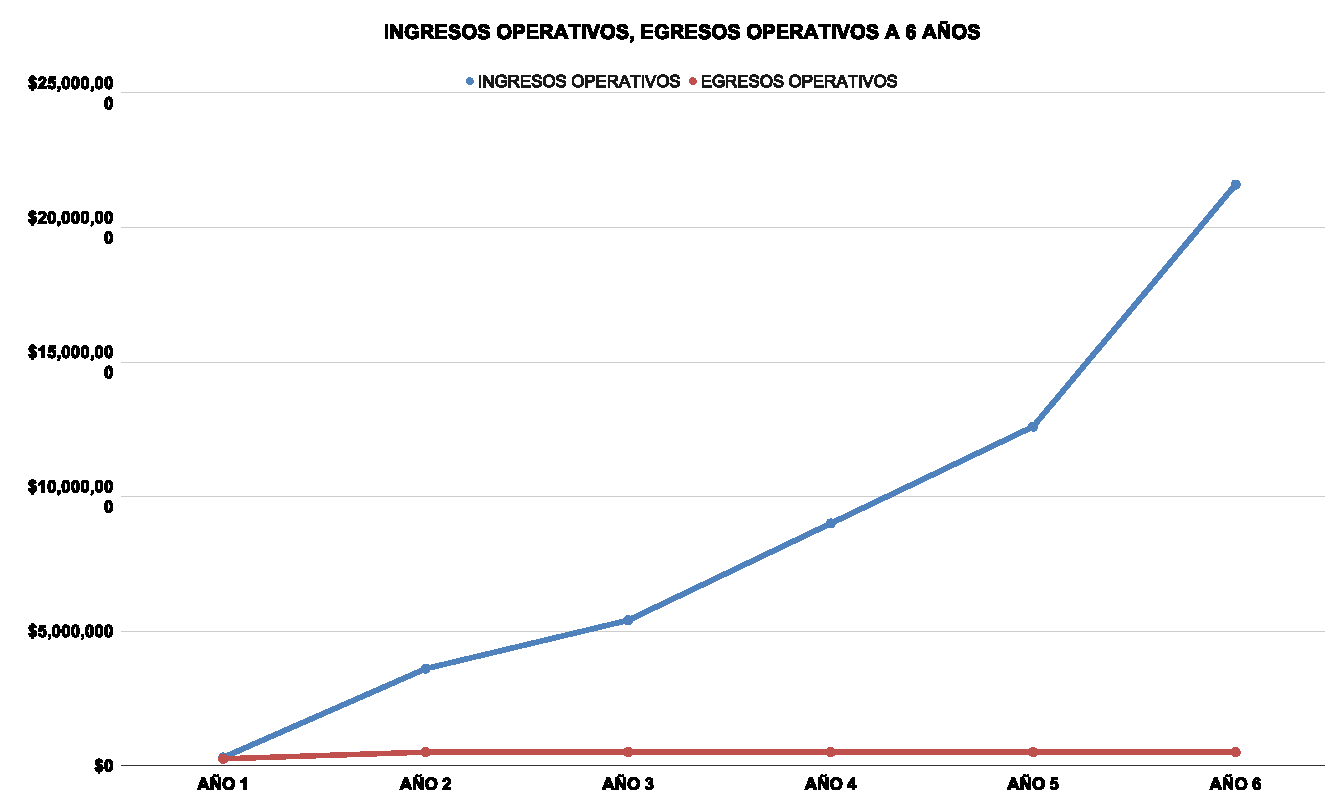
\includegraphics[height=0.28\textheight]{img/flujo_años_grafico.pdf}}
                \caption{Gráfico de flujo de caja correspondiente a los primeros seis años.}
                \label{fig:flujo_anios}
            \end{figure}

    \phantomsection     
    \section{Gestión de riesgos}

        \phantomsection
        \subsection{Criterios de ponderación}
            
            Para realizar el análisis de riesgos del proyecto, se toma como parámetros de evaluación a los siguientes criterios. En primer lugar, se contempla la probabilidad de ocurrencia de los riesgos mostrada en la Tabla~\ref{riesgos_prob}.
    
                \begingroup \setstretch{1.1}
                \begin{longtblr}[
                    caption = Escala de probabilidad de ocurrencia de riesgos,
                    label = riesgos_prob
                    ]{
                        colspec = {Q[c,m,2.5cm] Q[c,m,2.5cm] X[l,m]},
                        cells = {font=\small},
                        row{1} = {bg=gray!15, font=\small\bfseries, halign=c},
                        hlines, vlines,
                        rowsep = 3pt, colsep = 5pt
                    }
            
                        Cualitativa & Cuantitativa & Descripción \\ 
                        
                        Recurrente  & 5 & Este riesgo ocurrirá en algún momento \\
                        Probable    & 4 & Existe una gran probabilidad de que este riesgo ocurra \\
                        Posible     & 3 & Este riesgo podría ocurrir o no, probabilidades de 50/50 \\
                        Inusual     & 2 & Existe una gran probabilidad de que este riesgo no ocurra \\
                        Remota      & 1 & El hecho de que este riesgo ocurra es una posibilidad remota \\
            
                \end{longtblr}
                \endgroup
        
            Por otro lado, la gravedad de los mismos dada por la Tabla~\ref{riesgos_grav}.
    
                \begingroup \setstretch{1.1}
                \begin{longtblr}[
                    caption = Escala de gravedad de ocurrencia de riesgos,
                    label = riesgos_grav
                    ]{
                        colspec = {Q[c,m,2.5cm] Q[c,m,2.5cm] X[l,m]},
                        cells = {font=\small},
                        row{1} = {bg=gray!15, font=\small\bfseries, halign=c},
                        hlines, vlines,
                        rowsep = 3pt, colsep = 5pt
                    }
            
                        Cualitativa & Cuantitativa & Descripción \\ 
                        
                        Catastrófica & 5 & Las consecuencias de este riesgo serán muy perjudiciales y puede resultar difícil recuperarse \\
                        
                        Importante & 4 & Las consecuencias de este riesgo serán significativas y pueden causar daños a largo plazo \\
                        
                        Moderada & 3 & Las consecuencias del riesgo tardarán en mitigarse \\
                        
                        Menor & 2 & Las consecuencias del riesgo se gestionarán con facilidad \\
                        
                        Insignificante & 1 & El riesgo generará pocas consecuencias si ocurriera \\
            
                \end{longtblr}
                \endgroup
    
            A partir de estos criterios es posible calcular el impacto de los riesgos realizando la multiplicación de la probabilidad por la gravedad, la escala del impacto se observa en la Tabla~\ref{riesgos_imp}.
            
                \begingroup \setstretch{1.1}
                \begin{longtblr}[
                    caption = Escala de impacto de riesgos considerando probabilidad y gravedad,
                    label = riesgos_imp
                    ]{
                        colspec = {X[c,m] X[c,m] X[c,m] X[c,m] X[c,m] X[c,m]},
                        cells = {font=\small},
                        row{1} = {bg=gray!15, font=\small\bfseries, halign=c},
                        column{1} = {bg=gray!15, font=\small\bfseries},
                        cell{2}{2,3,4} = {bg=red!25}, cell{2}{5} = {bg=orange!30}, cell{2}{6} = {bg=green!25},
                        cell{3}{2,3} = {bg=red!25}, cell{3}{4,5} = {bg=orange!30}, cell{3}{6} = {bg=green!25},
                        cell{4}{2} = {bg=red!25}, cell{4}{3,4} = {bg=orange!30}, cell{4}{5,6} = {bg=green!25},
                        cell{5}{2,3} = {bg=orange!30}, cell{5}{4,5,6} = {bg=green!25},
                        cell{6}{2,3,4,5,6} = {bg=green!25},
                        hlines, vlines,
                        rowsep = 3pt, colsep = 5pt
                    }
                
                                & Catastrófica & Importante & Moderada & Menor & Insignificante \\
                    Recurrente  & 25 & 20 & 15 & 10 & 5 \\
                    Probable    & 20 & 16 & 12 & 8  & 4 \\
                    Posible     & 15 & 12 & 9  & 6  & 3 \\
                    Remota      & 10 & 8  & 6  & 4  & 2 \\
                    Inusual     & 5  & 4  & 3  & 2  & 1 \\
                
                \end{longtblr}
                \endgroup
        
            La clasificación del impacto se realiza de la siguiente forma:
    
                \begin{itemize}
                    \item \textbf{Bajo (0 al 7):} Es probable que los eventos de bajo riesgo no sucedan y, si suceden, no tendrán consecuencias relevantes para el proyecto. Baja prioridad en el plan de gestión de riesgos.
    
                    \item \textbf{Medio (8 al 13):} Los eventos de riesgo medio son una molestia y pueden causar contratiempos en el proyecto. No se deben ignorar estos riesgos, pero tampoco es necesario que sean la principal prioridad.
    
                    \item \textbf{Alto (14 al 25):} Si no se los tiene en cuenta durante la planificación del proyecto, los eventos de alto riesgo pueden hacer que el proyecto fracase. Dado que es probable que estos riesgos ocurran y tengan consecuencias graves, son lo más importante en el plan de gestión de riesgos.
                \end{itemize}

        \phantomsection
        \subsection{Riesgos identificados}
    
            Con base en lo mencionado anteriormente, se identificaron los riesgos y su impacto en el proyecto como se puede observar en la Tabla~\ref{riesgos}.

                \vspace{0.2 cm}
                \begingroup \setstretch{1.1}
                \begin{longtblr}[
                    caption = Riesgos y clasificación de los mismos,
                    label = riesgos
                    ]{
                        colspec = {Q[c,m,1cm] X[l,m] Q[c,m,2cm] Q[c,m,2cm] Q[c,m,2cm] Q[c,m,2cm]},
                        cells = {font=\small},
                        row{1} = {bg=gray!15, font=\small\bfseries, halign=c},
                        hlines, vlines,
                        rowsep = 3pt, colsep = 5pt
                    }
            
                        ID & Riesgo identificado & Ocurrencia & Gravedad & Impacto & Riesgo \\ 
                        
                        R1 & Sesgo y falta de generalización      & 3 & 5 & 15 & Alto  \\
                        R2 & Incompatibilidad de formatos         & 4 & 4 & 20 & Alto  \\
                        R3 & Dificultades con los datos locales   & 4 & 5 & 25 & Alto  \\
                        R4 & Fallas en la integración             & 4 & 2 & 8  & Medio \\
                        R5 & Subestimación de costos              & 4 & 3 & 12 & Medio \\
                        R6 & Demora de la certificación           & 3 & 2 & 6  & Bajo  \\
                        R7 & Resistencia de adopción              & 3 & 2 & 6  & Bajo  \\
                        R8 & Diferencias entre los integrantes    & 2 & 1 & 2  & Bajo  \\
            
                \end{longtblr}
                \endgroup
    
        \subsubsection*{Descripción de los riesgos}
    
            \begin{enumerate}[label=\textbf{R\arabic* - }] 
            
                \item \textbf{Sesgo y falta de generalización (Alto)}
                
                    El modelo de inteligencia artificial podría no mantener su eficacia al analizar topografías corneales de pacientes locales, debido a que su entrenamiento inicial se basó predominantemente en \textit{datasets} internacionales, generando falsos negativos o diagnósticos imprecisos.
    
                \item \textbf{Incompatibilidad de formatos (Alto)}
                
                    Riesgo de que los equipos topográficos o tomográficos de las clínicas exporten los estudios en formatos propietarios cerrados, anómalos o con resoluciones variables que el \textit{pipeline} de preprocesamiento del software no pueda interpretar adecuadamente.
    
                \item \textbf{Dificultades con los datos locales (Alto)}
                
                    Dificultad o incapacidad para recolectar las muestras topográficas de centros de salud de Misiones en los plazos establecidos, ya sea por falta de tiempo de los médicos colaboradores o por trabas en el proceso de anonimización, bloqueando la fase de validación clínica local.
    
                \item \textbf{Fallas en la integración (Medio)}
                
                   Aparición de errores técnicos, cuellos de botella o incompatibilidades de software al momento de acoplar el modelo de inferencia (\textit{backend/Python}) con la interfaz de usuario (\textit{frontend/React}) y montarlos de forma conjunta en el servidor VPS.
    
                \item \textbf{Subestimación de costos (Medio)}
                
                   Probabilidad de que el presupuesto planificado se vea superado por variaciones económicas reales, como incrementos imprevistos en las suscripciones a servicios Cloud (Google Colab, VPS), honorarios médicos o     aranceles regulatorios.
    
                \item \textbf{Demora de la certificación (Bajo)}
                
                  Posibilidad de sufrir retrasos burocráticos o administrativos durante el proceso de inscripción y auditoría, lo que postergaría el uso clínico formal del producto sin detener su desarrollo técnico.
    
                \item \textbf{Resistencia de adopción (Bajo) }
                
                  Desconfianza o falta de predisposición por parte de algunos oftalmólogos y técnicos locales para incorporar un sistema de IA como segunda opinión, prefiriendo sus métodos tradicionales y limitando el alcance de las pruebas operativas.
    
                \item \textbf{Diferencias entre los integrantes (Bajo)} 
                
                  Posibles desacuerdos técnicos, de criterio o de disponibilidad de horarios entre los miembros del equipo desarrollador, lo que podría generar pequeñas fricciones o ralentizar momentáneamente el avance de ciertas tareas.
                
            \end{enumerate}

        \phantomsection
        \subsection{Planes de acción}
    
            \begin{enumerate}[label=\textbf{R\arabic* - }] 
            
                \item \textbf{Sesgo y falta de generalización (Alto)}
                
                    \textbf{Mitigación:} Se implementarán técnicas de \textit{Data Augmentation} (aumento de datos) para enriquecer artificialmente las muestras locales disponibles, mejorando la robustez del modelo de \textit{Deep Learning}. Además, se implementará seguimiento al entrenamiento para prevenir \textit{overfitting} y \textit{underfitting} de los datos internacionales disponibles así como reentrenamiento continuo y monitoreo de deriva.
    
                    \textbf{Contingencia:} En caso de detectar un alto índice de falsos negativos durante las pruebas, se programarán sesiones intensivas con el oftalmólogo consultor para analizar exclusivamente los mapas de calor (XAI) de los casos erróneos. Esto permitirá identificar qué patrones morfológicos sutiles está ignorando la IA para proceder a un reentrenamiento focalizado y ajuste de la clasificación.
    
                \item \textbf{Incompatibilidad de formatos (Alto)}
    
                    \textbf{Mitigación:} Desde las fases iniciales, se solicitarán muestras de prueba de los distintos equipos disponibles en el mercado local (Pentacam). Con base en estas muestras, se construirá un \textit{pipeline} de preprocesamiento robusto en Python utilizando herramientas de visión artificial.
    
                    \textbf{Contingencia:} Si se detectan resoluciones anómalas o escalas de color propietarias que rompan la segmentación, el módulo de preprocesamiento se actualizará para forzar una estandarización (recorte, redimensionamiento y normalización de canales) antes de que la imagen ingrese al modelo predictivo, asegurando así la interoperabilidad del sistema.
                
                \item \textbf{Dificultades con los datos locales (Alto)}
    
                    \textbf{Mitigación:} Se desarrollará y entregará a los oftalmólogos colaboradores un \textit{script} automatizado y sencillo que elimine de manera instantánea los metadatos (información del paciente) de las imágenes exportadas. Esto reducirá drásticamente la carga de trabajo administrativo para ellos al momento de anonimizar las muestras.
    
                    \textbf{Contingencia:} Si un único centro médico no logra alcanzar la cuota de imágenes necesarias en el tiempo estimado, se ampliará inmediatamente la solicitud de colaboración a otras clínicas oftalmológicas o centros de alta complejidad ubicados en los principales núcleos urbanos de la provincia de Misiones (como Posadas, Oberá y Eldorado).
                
                \item \textbf{Fallas en la integración (Medio)}
    
                    \textbf{Mitigación:} El desarrollo se realizará de manera estrictamente modular. Se construirán y probarán de forma aislada los \textit{endpoints} de la API en el \textit{backend} antes de conectarlos a la interfaz gráfica desarrollada en React.
    
                    \textbf{Contingencia:} Se utilizarán tecnologías de contenerización (como Docker) para encapsular la aplicación. De este modo, si surgen incompatibilidades al migrar el sistema desde las computadoras de desarrollo local hacia el servidor VPS, el contenedor garantizará que el entorno de ejecución sea exactamente el mismo, aislando el problema rápidamente.
                       
                \item \textbf{Subestimación de costos (Medio)}
    
                    \textbf{Mitigación:} Se llevará un control estricto de los gastos operativos y se optimizará el uso de la infraestructura en la nube (activando los recursos de pago como Google Colab Pro solo en periodos críticos). Para contener los gastos en honorarios médicos durante la auditoría de datos, se buscará establecer convenios de colaboración académica con los especialistas locales, ofreciendo coautoría en publicaciones científicas a cambio de su asesoramiento experto.
    
                    \textbf{Contingencia:} En caso de que los aranceles regulatorios (como la habilitación de empresa y registro del producto médico ante la ANMAT) superen la capacidad financiera del proyecto, se buscará una asociación estratégica con una institución médica o empresa tecnológica que ya posea la habilitación legal correspondiente. Alternativamente, la primera versión se podría distribuir como software de uso para investigación (\textit{Research Use Only}) sin validez diagnóstica comercial, lo que evitará los altos costos de registro inicial hasta que se consiga financiamiento externo o rondas de inversión.
                    
            \end{enumerate}

        \phantomsection
        \subsection{Impacto temporal}

            La materialización de los riesgos identificados afecta de forma distinta al cronograma del proyecto, existiendo casos donde el impacto es directo, otros donde es indirecto o acotado, y otros donde no compromete la planificación técnica.
            
            En el caso de \textbf{R1 (Sesgo y falta de generalización)}, si se detecta durante la etapa de validación clínica, la contingencia de reentrenamiento focalizado implicaría un retroceso hacia la etapa de desarrollo, extendiendo su duración original. De forma similar, \textbf{R2 (Incompatibilidad de formatos)} puede afectar el cronograma en dos momentos distintos: durante el desarrollo, si obliga a reconstruir el módulo de preprocesamiento antes de continuar con el entrenamiento, o durante la validación clínica local, si algún centro de salud utiliza un equipo con un formato no contemplado originalmente, retrasando el inicio de esa etapa. 
            
            \textbf{R3 (Dificultades con los datos locales)} constituye el caso más directo, ya que su propia definición está condicionada por los plazos de recolección y su materialización bloquea explícitamente el comienzo de la etapa de validación clínica local hasta resolverse. En contraste, \textbf{R4 (Fallas en la integración)} presenta un impacto temporal acotado, dado que el desarrollo modular y la contenerización mediante Docker permiten aislar y resolver los errores rápidamente sin detener el avance general del proyecto. 
            
            \textbf{R5 (Subestimación de costos)} impacta principalmente en lo financiero y no en el cronograma técnico de desarrollo. Sin embargo, puede generar una afectación indirecta si se activa su contingencia, ya que gestionar una asociación estratégica o una ronda de financiamiento externo consume tiempo adicional que podría postergar puntualmente la etapa de certificación regulatoria y lanzamiento.
            
            \textbf{R6 (Demora de la certificación)} no afecta el cronograma de desarrollo técnico, puesto que su propia descripción aclara que los retrasos burocráticos posponen únicamente el uso clínico formal y comercial del producto, permitiendo que el desarrollo continúe en paralelo. 
            
            \textbf{R7 (Resistencia de adopción)} recae más sobre el alcance que sobre el tiempo, reduciendo la cantidad de casos disponibles durante la validación en lugar de extender directamente su duración, salvo que sea necesario reclutar centros o profesionales adicionales, lo que generaría una demora acotada. 
            
            Finalmente, \textbf{R8 (Diferencias entre los integrantes)} sí presenta una afectación sobre el cronograma según su propia descripción, aunque de carácter menor, puntual y limitado a tareas específicas del equipo, sin comprometer las etapas generales del proyecto.

            En conclusión, los riesgos con afectación directa y relevante sobre el cronograma son \textbf{R1, R2 y R3}, los riesgos con afectación indirecta o acotada son \textbf{R4, R5, R7 y R8}, mientras que \textbf{R6} es el único riesgo que no compromete en ningún grado el desarrollo técnico ni su cronograma.

            Cabe destacar que la validación clínica con muestras locales forma parte de la proyección del producto, por lo que R1 y R3 no bloquean la entrega del PFI: si las muestras se obtienen durante el PFI, se incorporan a una primera evaluación del modelo; de lo contrario, el prototipo se evalúa sobre el conjunto de datos público. Para los riesgos que sí pueden afectar al PFI, como R2, R4 y R8, así como para las iteraciones propias del modelado, el cronograma prevé la reserva de contingencia de hasta dos meses descrita en la Propuesta metodológica.